\chapter{Solver Parameter Testing}
\label{solvtestchap}

% TODO[X] move preface and rhoreactingfoam stuff into OF det modeling section

% TODO[X] start with setup of rrcf and move Sod into previous 

% TODO[X] 4.3 basically consumes this chapter 

%\section{Preface}

%This chapter will go through progression of research on efficacy for the different solvers and detonation modeling techniques performed during the duration of this thesis work. In an effort to assist the University of Colorado's Turbulence and Energy Systems Laboratory (TESLa), several solvers and methods will be tested for potential for detonation modeling, stability, and accuracy, typically in that order. Additional focus will be on the effects of AMR on the results. 


Now that \verb|rhoReactingCentralFoam| has been selected for use, the solver can be tested further to determine how different selections in solver parameters alter the solution. Parameters that were tested are the Arrhenius equations's pre-exponential factor exponent, the Courant \cite{courant} number and time step variation, static mesh resolution, and adaptive mesh refinement variation. Sensitivities to certain solver parameters as well as mesh resolution on the solution were be explored. 


%\section{Solver Parameter Testing and Sensitivity}

\section{Ignition Tests}
\label{sec:igstudy}
The first necessary set of tests before solver and AMR parameters can be explored were those testing detonation ignition methods. Different ignition techniques can be used to start a detonation. Both the block ignition and gradient ignition methods were examined. 

\subsection{Block Ignition}

The block ignition method with high pressure and temperature stoichiometric reactants was utilized initially to build off the work done in \cite{towery1}. A rectangular region spanning from the ignition wall (y-z plane at \(x = 0\) m) to \(x = 0.001\) m was set with a different initial condition than the rest of the domain using the \verb|setFields| utility. The ignition block region contained high pressure and temperature reactants at 3000 K and 20 atm, with the rest of the domain at 300 K and 1 atm. This method is seen in Figure \ref{fig:blockig}.
\begin{figure}[h]
\centering
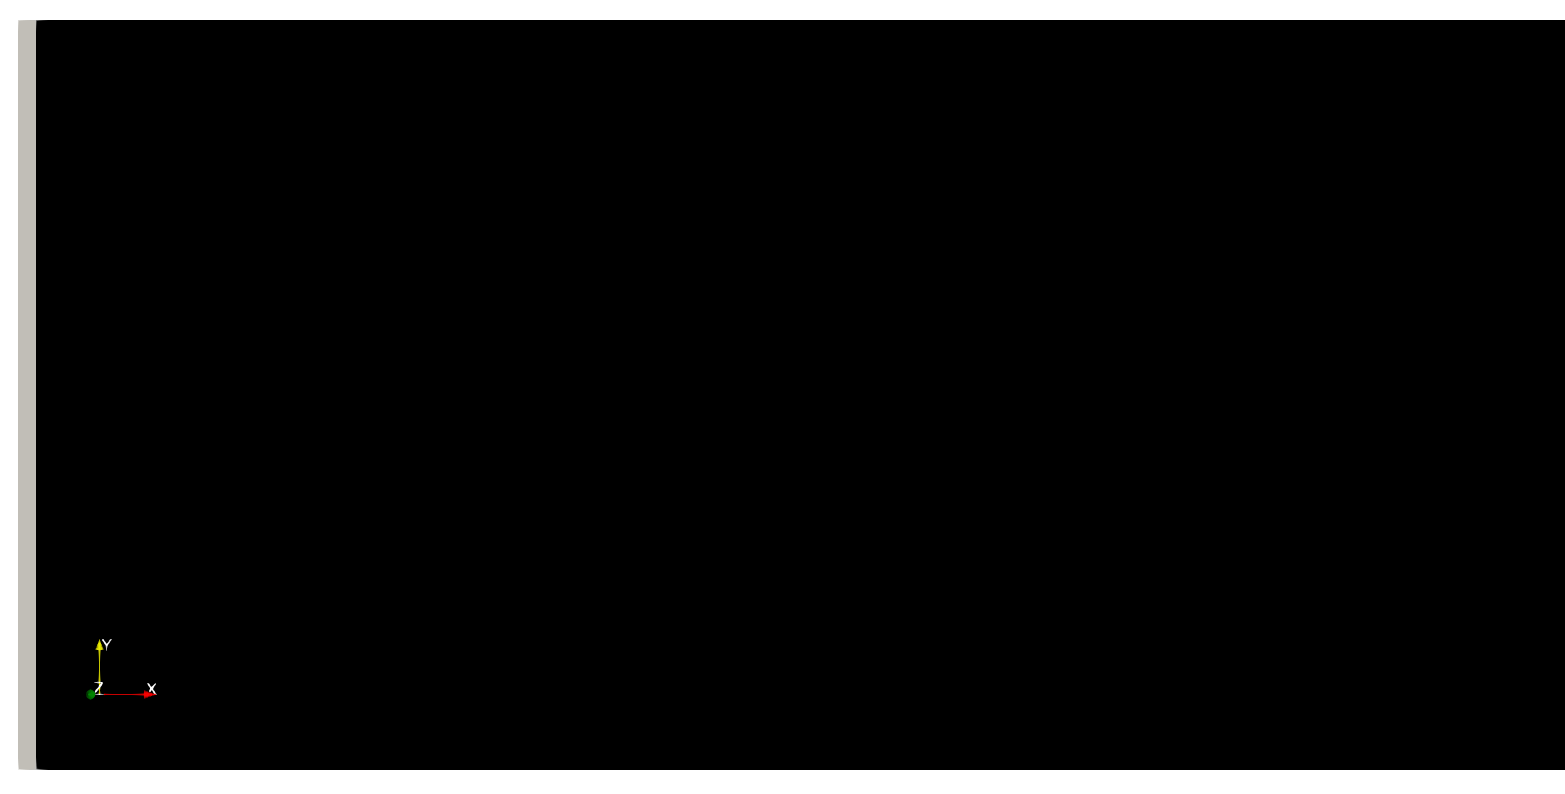
\includegraphics[width=0.8\textwidth]{figs/ignition/block.png}
\caption{Block ignition method, seen on left side of domain, at t = 0 s}
\label{fig:blockig}
\end{figure}%
\noindent Ultimately this ignition approach was not pursued further due to instability in detonation initiation due to the very large gradient in conditions between the block ignition region and the rest of the domain. For both very high and very low grid resolutions, detonation would sometimes not occur and instead the shockwave would decouple from the flame reaction front. A better approach shown by Towery\cite{towery2} is to use a pressure and temperature gradient ranging from the wall to the domain, smoothly transitioning the ignition region to the domain. 

\subsection{Gradient Ignition}
Using the theory shown in Towery \cite{towery2}, we developed an initial gradient ignition condition to guarantee a detonation across mesh resolutions. This gradient ignition spanned 0.01 m from the leftmost wall, ranging from 1200 K at the wall to the domain temperature of 300 K. \verb|setFields| cannot set fields for initial conditions with functions, so \verb|funkySetFields| was applied for the gradient condition. This can be seen in Figure \ref{fig:gradig}. 
\begin{figure}[h]
\centering
\includegraphics[width=0.8\textwidth]{figs/ignition/gradient.png}
\caption{Gradient ignition method, seen on left side of domain, at t = 0 s}
\label{fig:gradig}
\end{figure}%
\noindent After transitioning to this ignition method, detonations were less noisy and more consistent in their ignition. The next stage towards matching experimental results and other computational detonation modeling was to attempt to model detonation cells. 

\section{Cellular Detonation Modeling Attempts}
Comparison of cellular detonation structure is one method to validate numerical solvers with experimental results. Maximum pressure and density plots across all time steps for every cell can be plotted to emulate experimental ``smoke foil'' results. The smoke foil is a piece of smooth metal placed flat against a wall in a detonation tube chamber, in which smoke particles have been evenly distributed (usually by a fire) upon the surface of the foil. When a detonation passes over the smoke foil, the density and pressure differences will leave fish scale-like patterns upon the foil. 
In order to better match experimental conditions and form detonation cells, the temperature gradient initial condition was also expanded to include a randomized 240 K temperature increase throughout the domain seen in Figure \ref{fig:gradrand}. 
\begin{figure}[h]
\centering
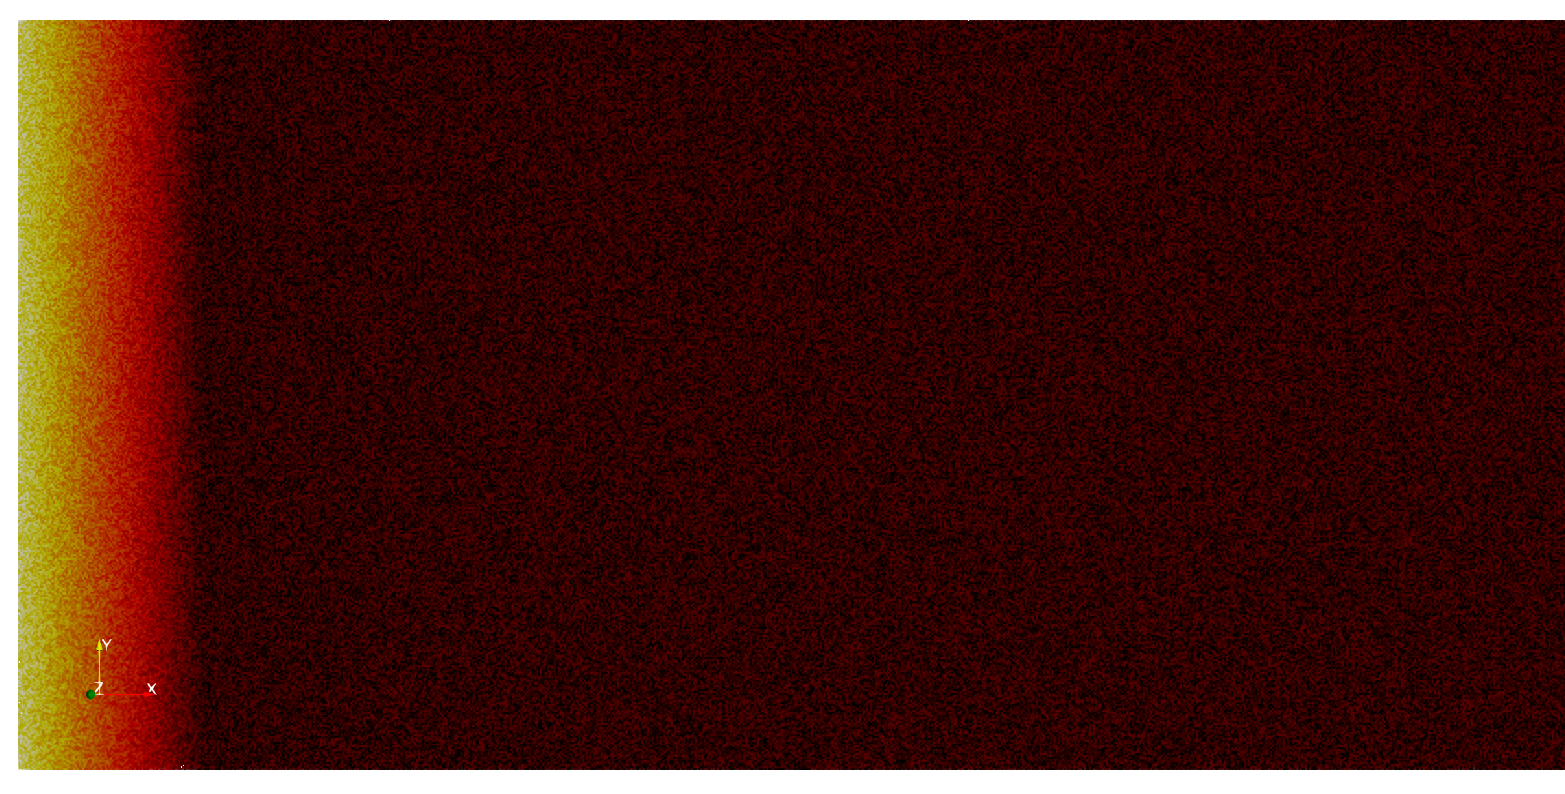
\includegraphics[width=0.8\textwidth]{figs/ignition/randgrad.png}
\caption{Gradient ignition method with randomized temperature distribution throughout domain, seen on left side of domain, at t = 0 s}
\label{fig:gradrand}
\end{figure}%
\noindent This was chosen as it is 20\% of the maximum initial ignition temperature, and should provide enough randomization to instantiate detonation cells. The randomization of temperature from +0 K to +240 K is uniform and not Gaussian in distribution. With the randomization of temperature throughout the domain, the maximum value of density across all time steps for each cell was recorded and plotted as a surface plot. 
%This plot type will emulate what is seen in experimental results using what is known as a ``smoke foil''.
For a 2500-400-1 mesh, this is seen in Figure \ref{fig:maxrho}.
\begin{figure}[h]
\centering
\includegraphics[width=0.9\textwidth]{figs/example_results/maxrho.png}
\caption{Surface plot of maximum density tracked across all time steps for each cell emulating a ``smoke foil''}
\label{fig:maxrho}
\end{figure}
From this figure, we deduced that detonation cells are possible but never initiated. The distinct cellular structure is not seen here, and further work with more accurate multi-step reaction mechanisms may have more success in bringing light to these features for detonations within \verb|rhoReactingCentralFoam|. Note that the field was not tracked for very long throughout the simulation due to the extreme data storage requirements for such thermodynamic field tracking. When ParaView is utilized to access the temporal statistics on a flow variable, very small time steps are required in order for the temporal statistical plots to not appear ``choppy'' and broken up. For the plot here, save files were required every \(1 \times 10^{ - 8}\) s in order to be continuous and smooth. With one million cells per time step, this quickly scales. However, detonation cells would be visible at this stage in the simulation as the detonation wave has stabilized. Other factors that may assist the formation of detonation cells are mesh resolution and the strength of the randomization parameters used throughout the flow field. When utilizing AMR, care must be used when attempting to model detonation cells since unrefinement behind the detonation wave smooths the solution considerably and flame structure as well as detonation cell formation may be eliminated. It is likely best to start with a static mesh and formulate the detonation cells to compare to experimental results, and then use the cell-structure-matched static mesh as a target for tuning AMR parameters. Different ranges of randomization throughout the flow field will also alter how the detonation front progresses and forms detonation cells. Another benefit of the addition of slight noise in the background domain is the ability to determine when the mesh resolution is refined enough to begin resolving fine detonation structure. As seen in the high refinement two-dimensional static mesh detonation results later in this chapter, the fine variation in the detonation wave itself is seen and therefore the threshold for resolving such structures is known. 



\section{Arrhenius Pre-exponential Factor}
\label{sec:a}

In order to better characterize reaction sensitivity and compare to other published results, testing was performed on the units of the pre-exponential factor for the Arrhenius equation in the \verb|reactions| file. Since the geometry, boundary, and initial conditions are all matched to the setup for the detonation tube in Towery\cite{towery1}, we will use the results there as a generic target to determine the order of magnitude of the exponent on the pre-exponential factor. The exponent was swept between \(10^{11}\) through \(10^{17}\). The results are seen in Figures \ref{fig:atestp}, \ref{fig:atestt}, and \ref{fig:atestu}. 

\begin{figure}
\centering
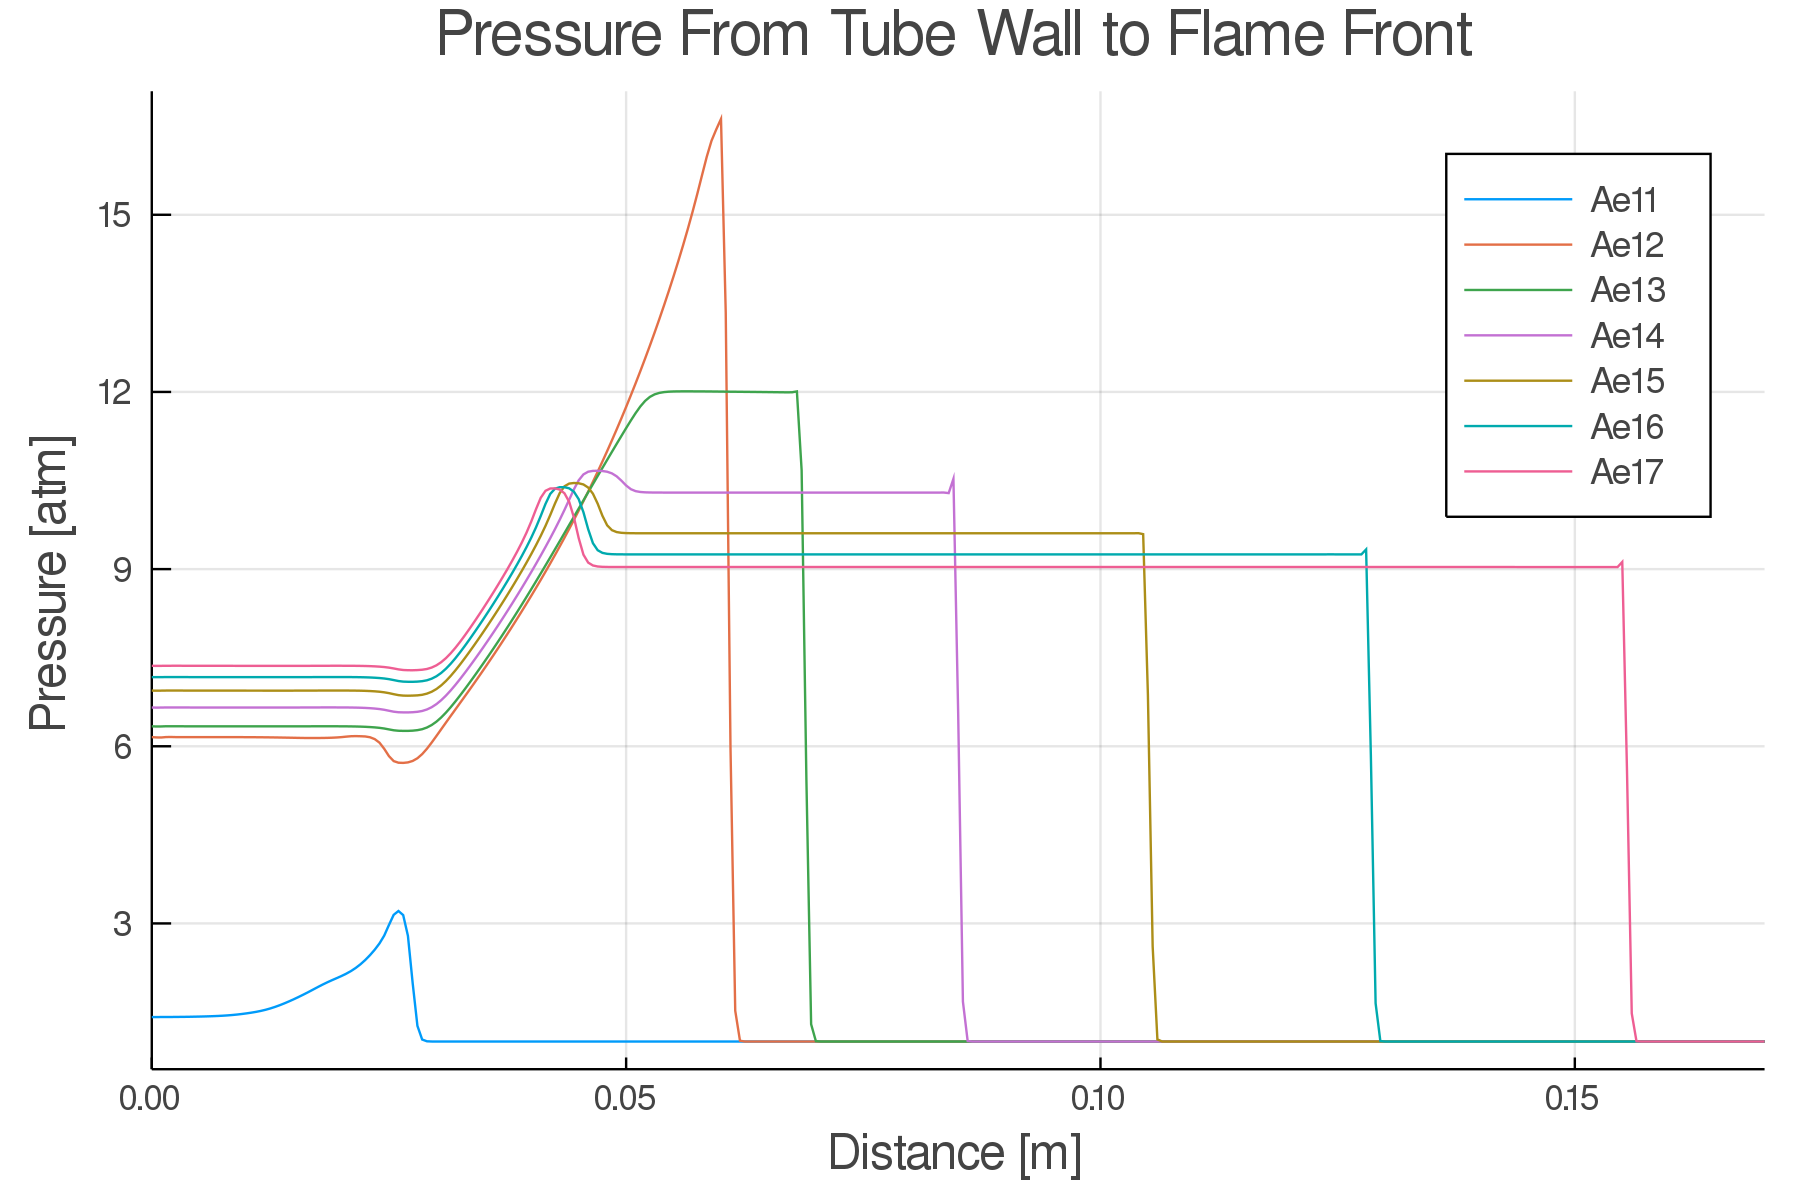
\includegraphics[width=0.85\linewidth]{./figs/Atest/p.png}
\caption{Pressure distribution in detonation tube for pre-exponential factor exponent sweep test}
\label{fig:atestp}
\end{figure}

\begin{figure}
\centering
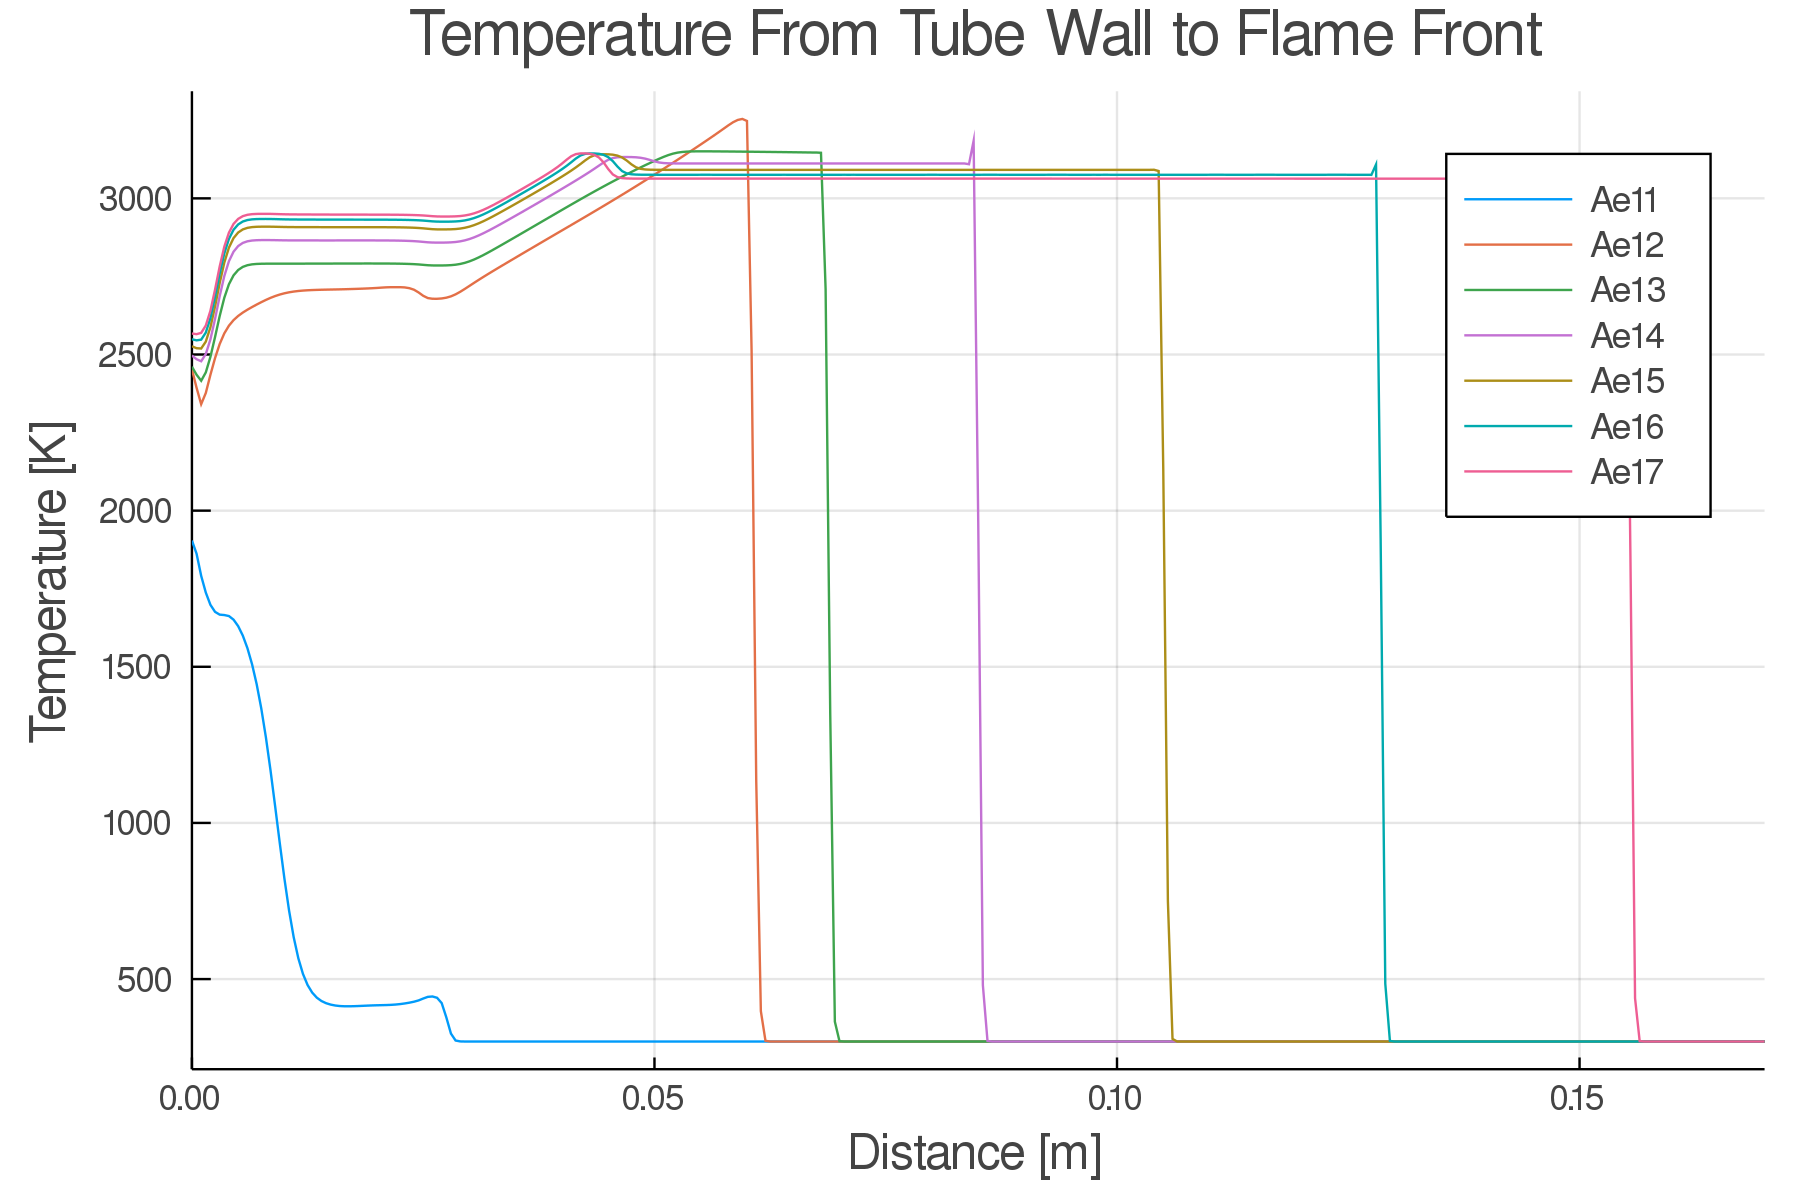
\includegraphics[width=0.85\linewidth]{./figs/Atest/t.png}
\caption{Temperature distribution in detonation tube for pre-exponential factor exponent sweep test}
\label{fig:atestt}
\end{figure}

\begin{figure}
\centering
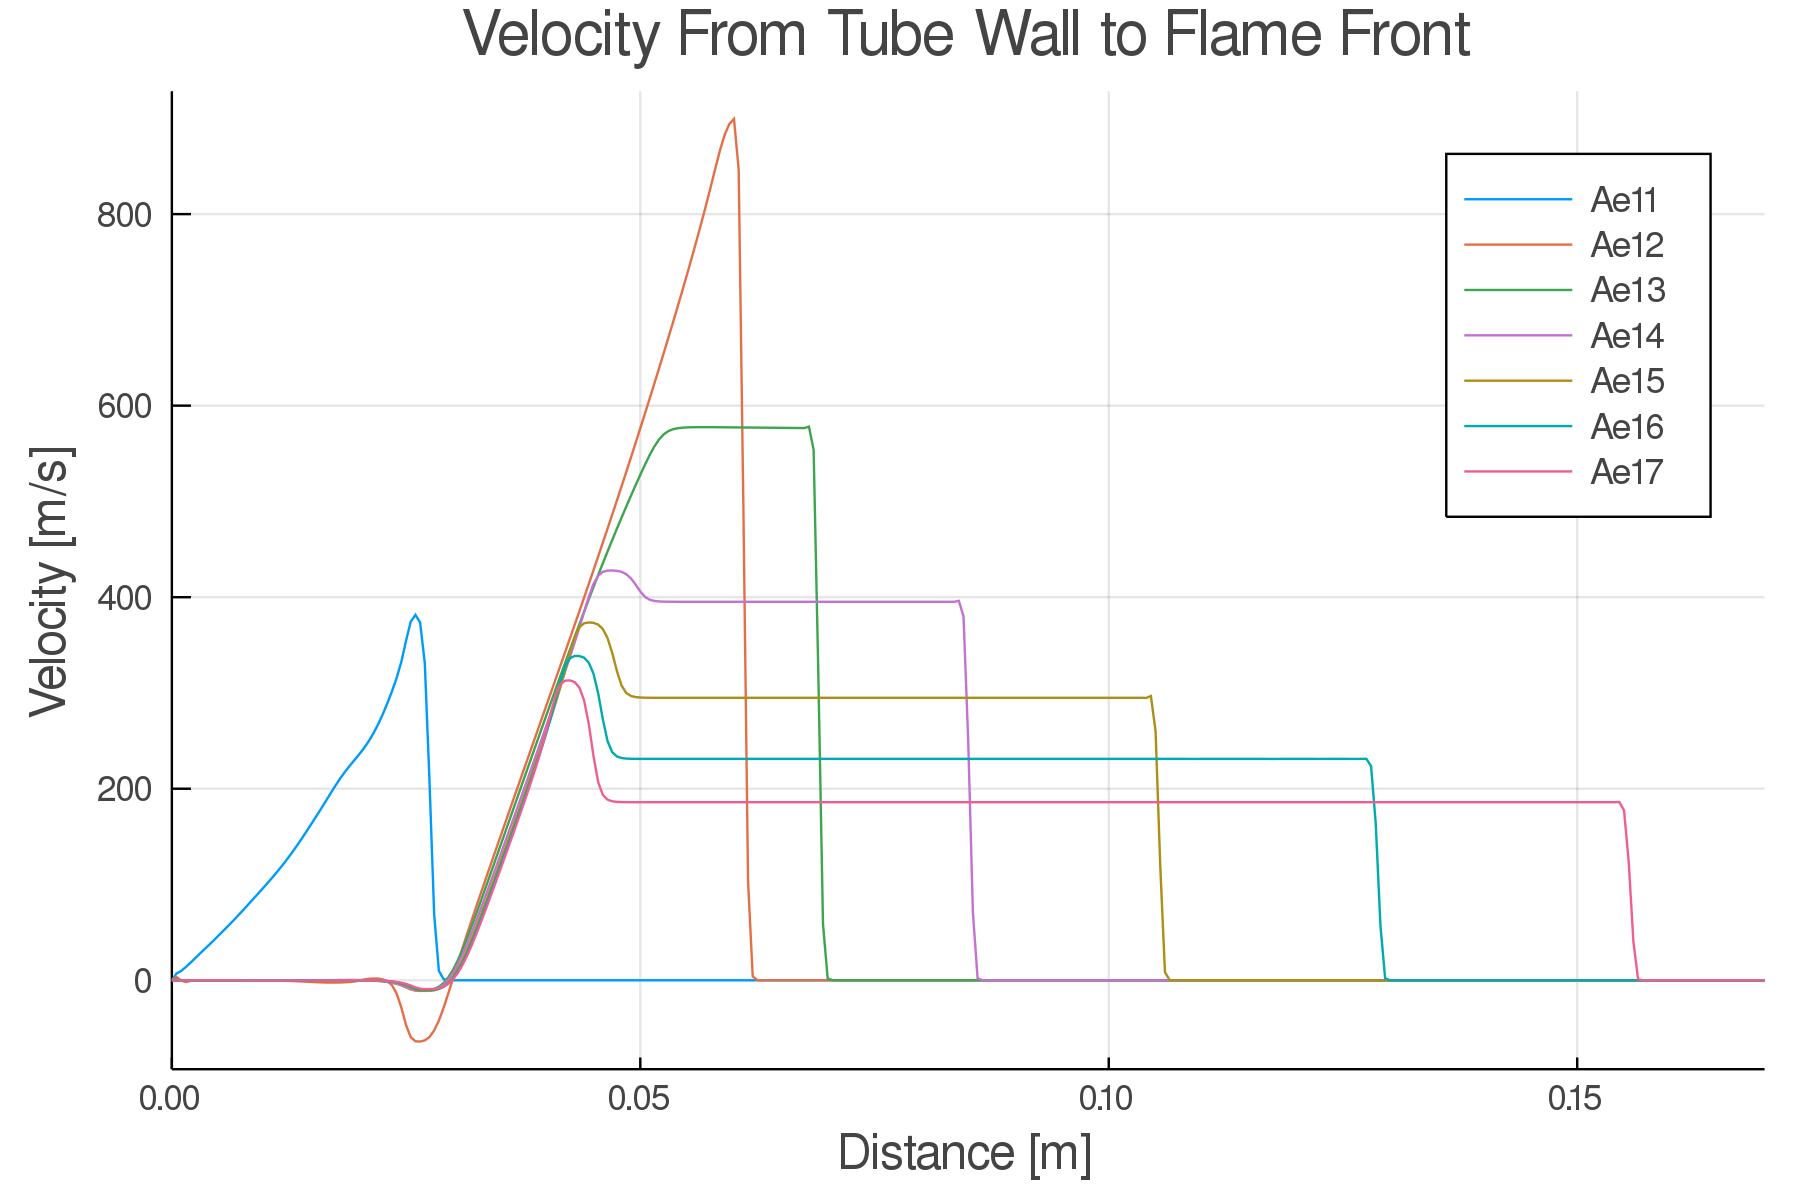
\includegraphics[width=0.85\linewidth]{./figs/Atest/u.png}
\caption{Velocity distribution in detonation tube for pre-exponential factor exponent sweep test}
\label{fig:atestu}
\end{figure}

From these figures, we can see the importance of having an accurate order of magnitude on the exponent for results. As the exponent was increased beyond the power of 12, plateaus emerge in the results for all thermodynamic variables. Under the power of 12, there is a large jump in solution, and a transition from between detonation states, seen in Figure \ref{fig:pjump}. The differences in these states is due to the coupling of the shockwave and the reactions (flame). The grouping of plots with higher pressure values have the reactions coupled with the shock, and the smaller pressure value grouping has the reaction occurring more slowly and trailing behind the shock. This is more evident in Figures \ref{fig:atestrp} and \ref{fig:atestrt} where we see that there is still a shockwave present in the ``lower'' group, but it is clear by Figure \ref{fig:atestrt} that the reaction process is happening much later than the shockwave instead right at the shock front. Thus presence of a shockwave in this scenario is not due to the sustained reaction, and was triggered by high pressure (and temperature) region used to initialize detonations in the simulation. 

\begin{figure}
\centering
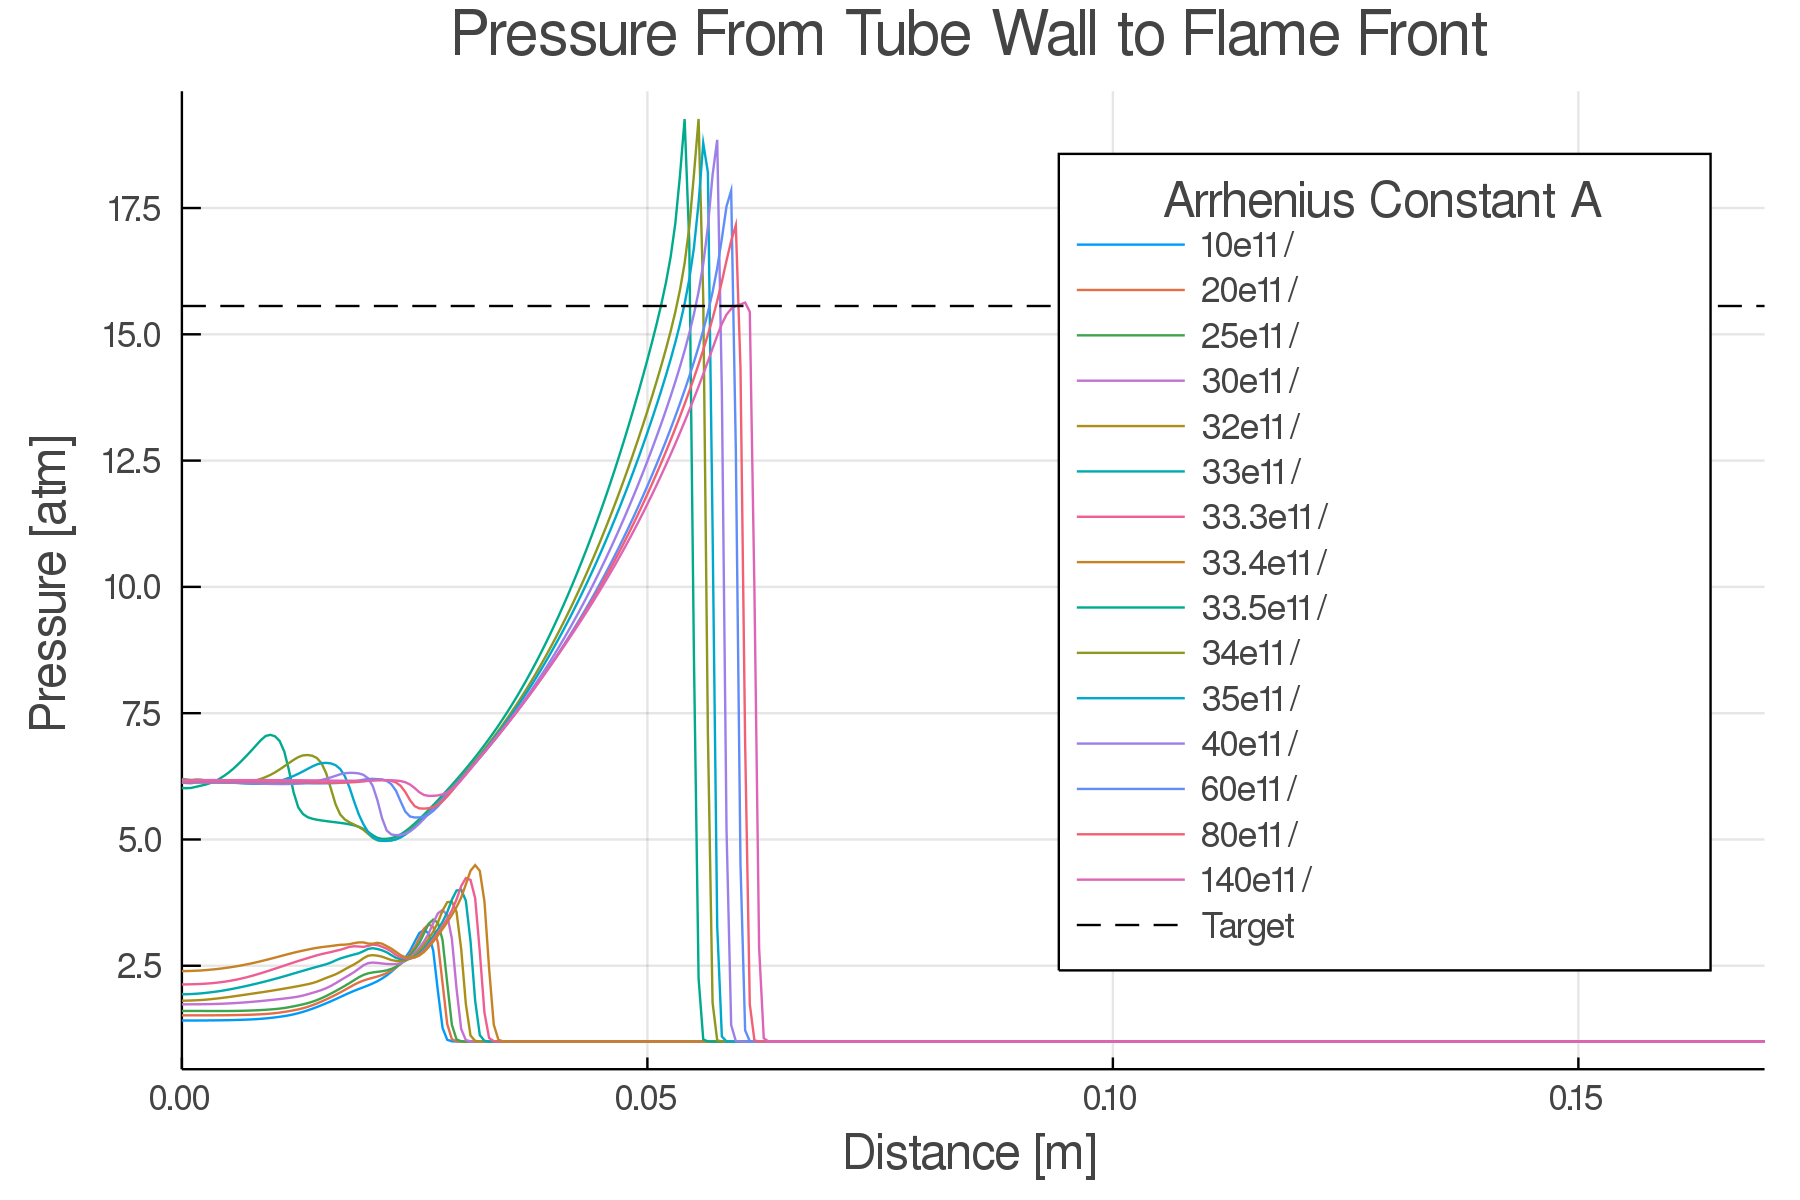
\includegraphics[width=0.85\linewidth]{./figs/Atest_refined/p_large.png}
\caption{Pressure distribution in detonation tube for expanded and refined pre-exponential factor exponent sweep test, showing detonation shock-reaction coupling transition. See Figures \ref{fig:atestrp} and \ref{fig:atestrt} for a filtered version.}
\label{fig:pjump}
\end{figure}


The exponent in this region was explored further since plateaus in thermodynamic properties values are not physical for real-world detonations. Note that the velocity plotted in Figure \ref{fig:atestu} is a fluid velocity, not a wave velocity. When instead we swept over a smaller interval, with the Chapman-Jouguet (CJ) targets from Towery\cite{towery1} plotted, we can see that there is a very abrupt transition in detonation stability (Figures \ref{fig:atestrp} and \ref{fig:atestrt}). 

\begin{figure}
\centering
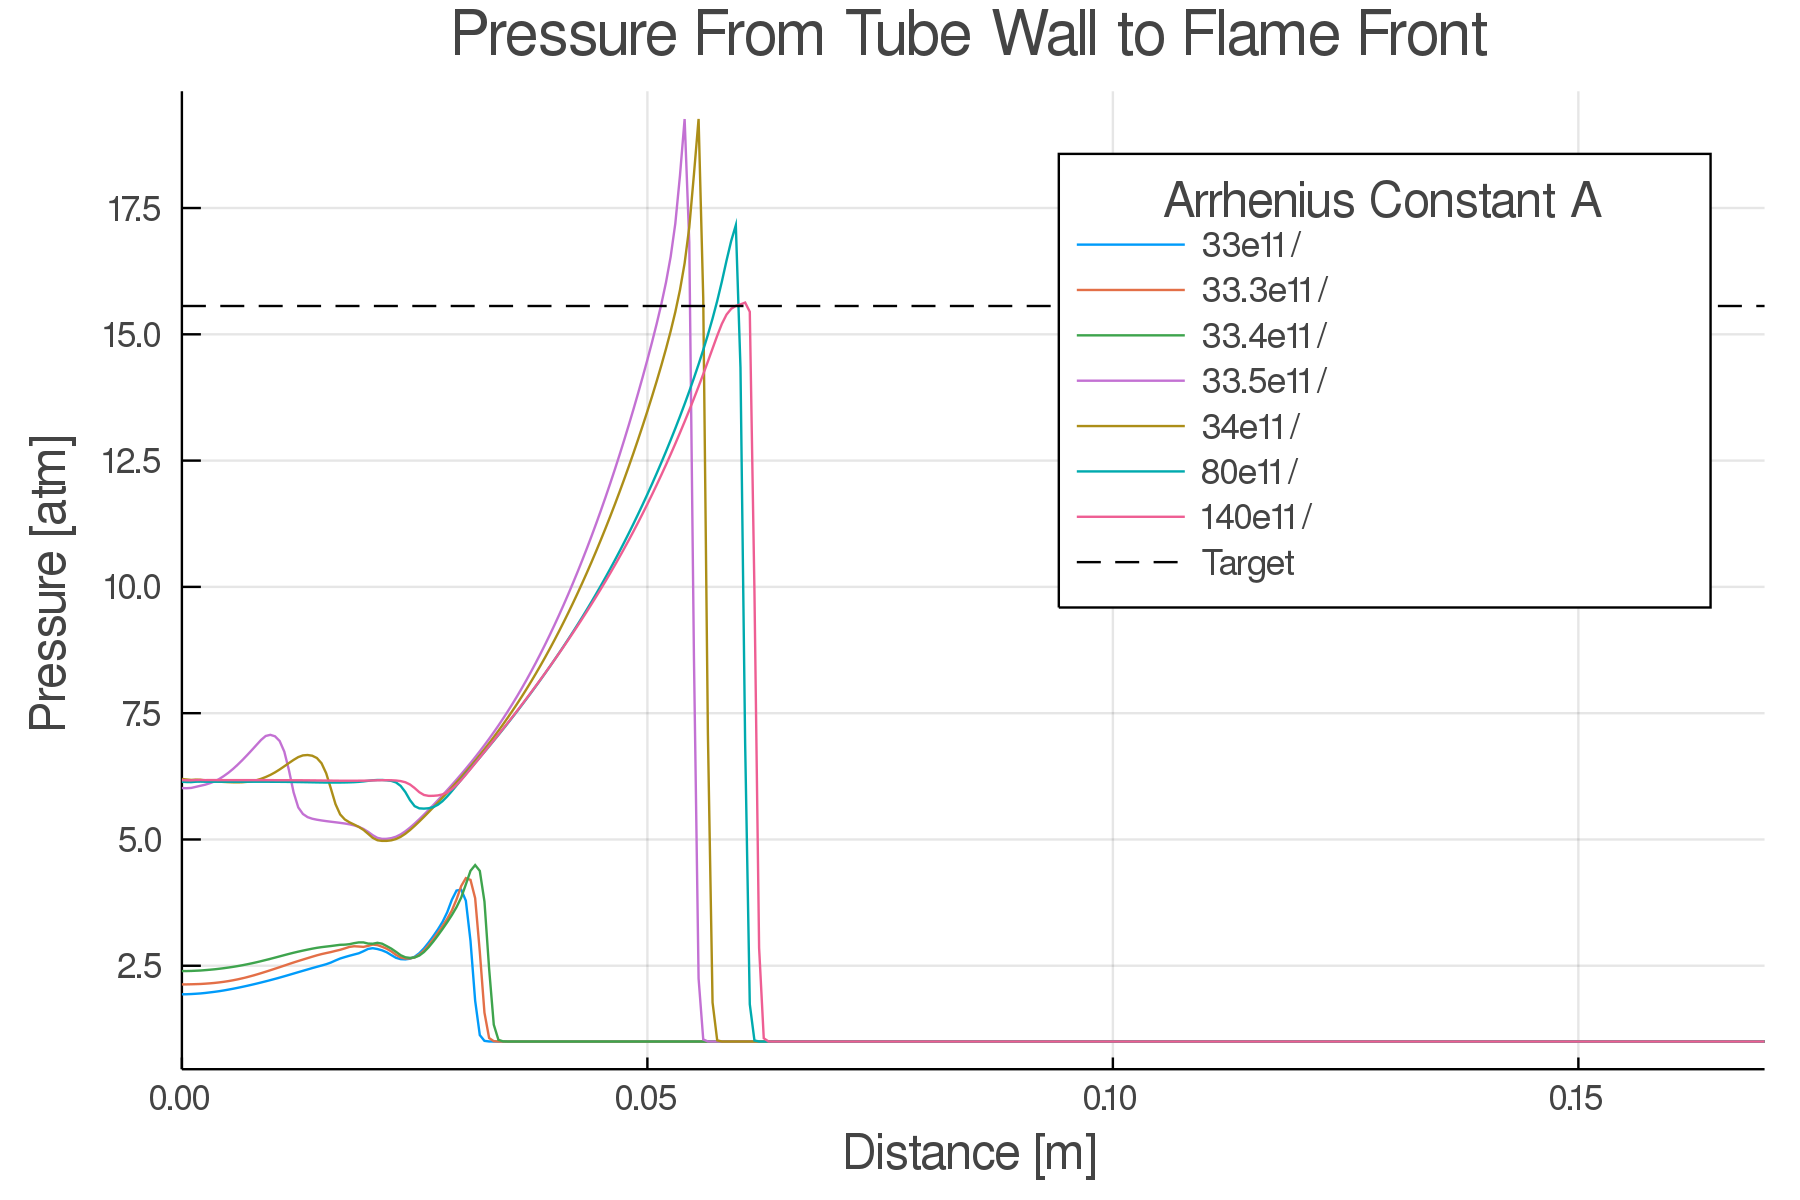
\includegraphics[width=0.85\linewidth]{./figs/Atest_refined/p.png}
\caption{Pressure distribution in detonation tube for refined pre-exponential factor exponent sweep test, filtered from Figure \ref{fig:pjump} and refined from Figure \ref{fig:atestp}}
\label{fig:atestrp}
\end{figure}

\begin{figure}
\centering
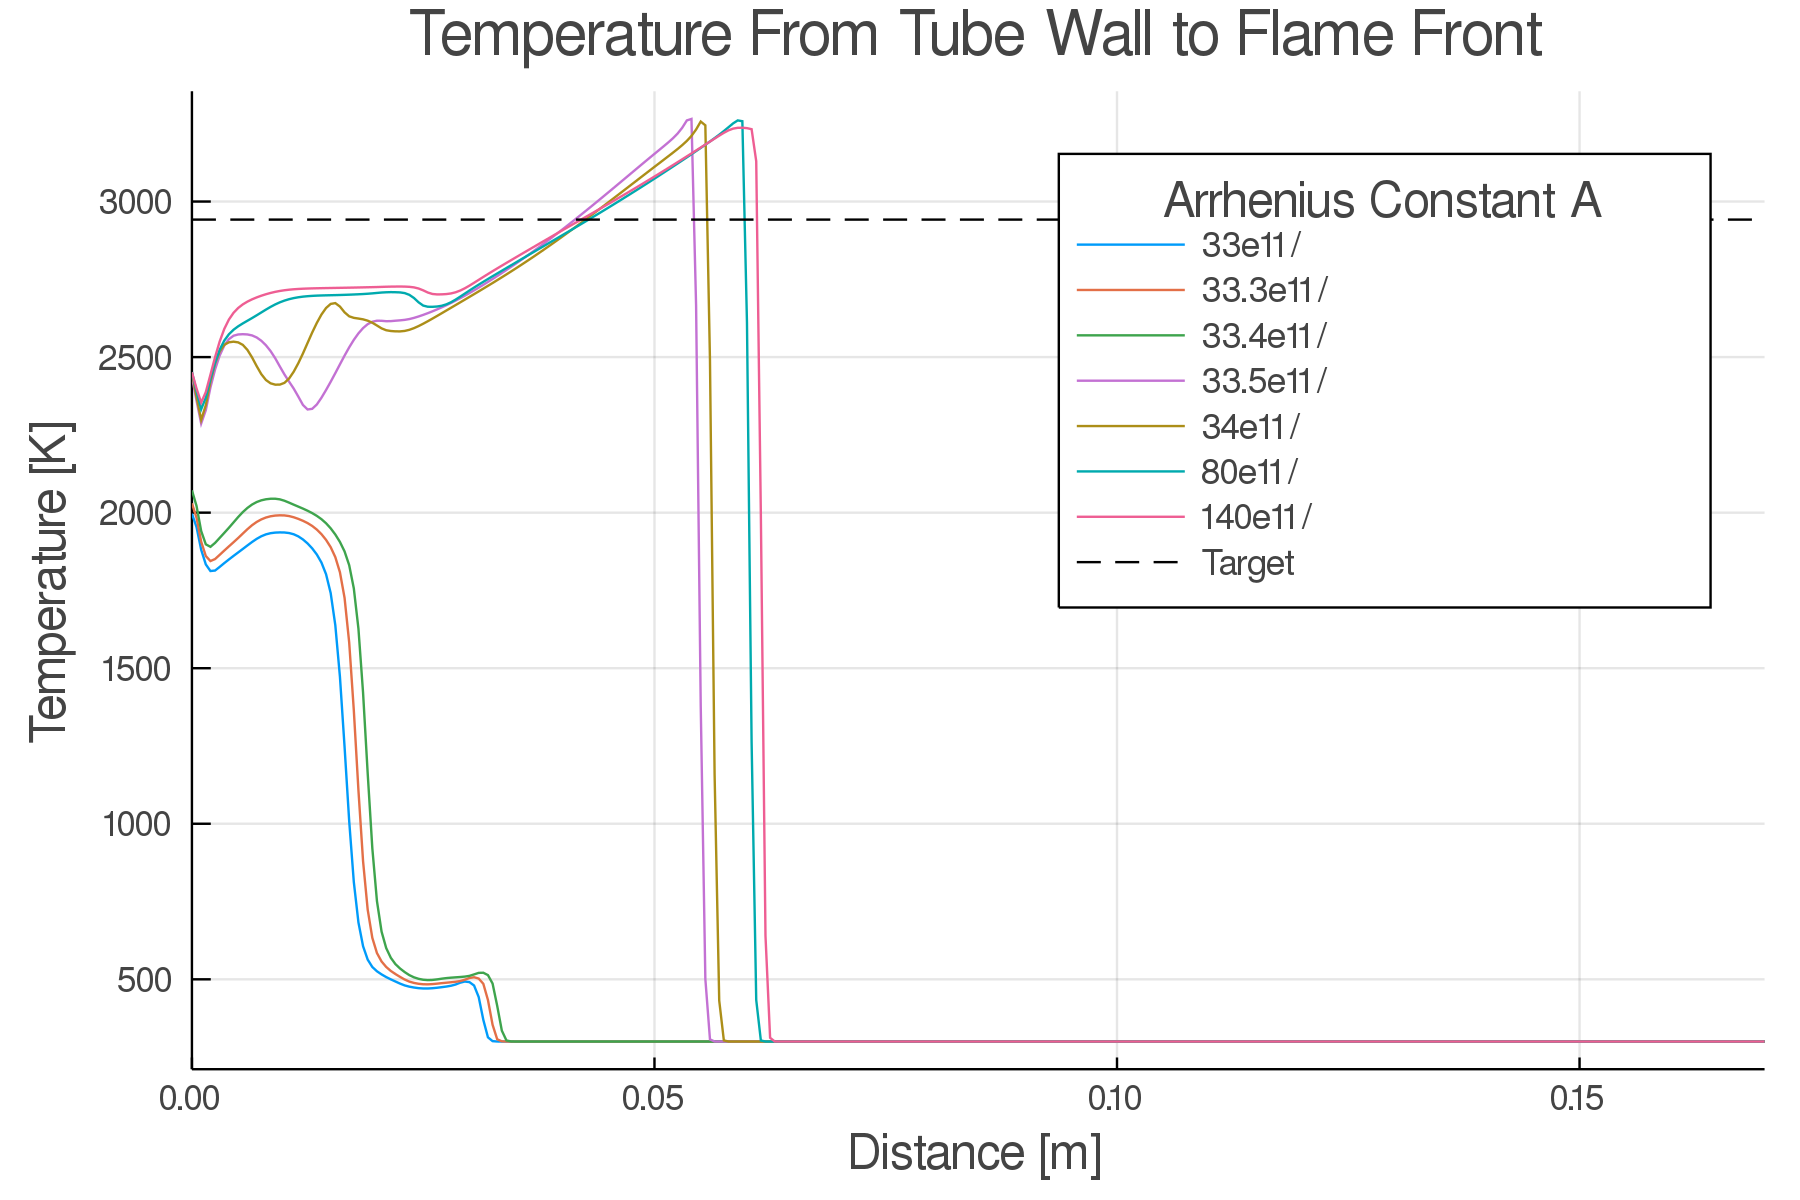
\includegraphics[width=0.85\linewidth]{./figs/Atest_refined/t.png}
\caption{Temperature distribution in detonation tube for refined pre-exponential factor exponent sweep test, refined from Figure \ref{fig:atestt}}
\label{fig:atestrt}
\end{figure}

With these tests, \(10^{13}\) was selected as an appropriate order of magnitude as it not only agreed with the results seen in Towery\cite{towery1}, but also with the value given for a single-step hydrogen-oxygen detonation in other published works\cite{hashemi}. 




\section{Time Step Variation}
One of the important tests was to determine how large the time step of the simulation could be taken. In OpenFOAM, one has several options for how the time step should be selected. By default, time steps are fixed, and set within \verb|controlDict|. Setting different values for how large the time step should be will affect the stability and solution of the simulation. Larger time steps will be more unstable, increasing the Courant number and sometimes leading towards the inability for solutions at a time step to converge. If we consider a fluid particle, the faster it moves, the more distance it can cover in a unit of time. If it is moving very quickly, large time steps mean this fluid particle could have traversed very far, leading to uncertainty in the solution. In a more general sense, we consider information and how it progresses throughout the gridded domain. For Courant numbers larger than one, the fluid is moving through more than one grid point per time step, and this is very difficult for the time integrators solving the flow equations to assess accurately. The logical choice would be to always select a very small time step to ensure a more stable and accurate solution. However, with decreased time step intervals comes increased computational cost, as the computer must solve the fluid equations much more often to arrive at a specific point in time. Instead, a smarter approach can be taken, where the time step is allowed to vary based on the Courant number. 

Inside \verb|controlDict| for \verb|rhoReactingCentralFoam|, we can set a maximum for both the typically-used fluid velocity Central Courant number as well as the acoustic (wave speed) Courant number. Each iteration, the solver will check the value of both these Courant numbers, and decrease the time step accordingly if the Courant number maximum is exceeded. In an effort to best determine how large the Courant number and therefore the time step can be, the maximum Courant number was set and swept across for various values. For these tests, a domain size of \( (x,y,z) = (0.5,0.04,0.04) \) meters was used with a 5000-3-3 mesh. This is pseudo-one-dimensional setup. Several maximum Courant (CFL) \cite{courant} numbers were swept across, and the results at \(3\times 10^{ - 5}\)s are plotted in Figures \ref{fig:cflp}, \ref{fig:cflt}, and \ref{fig:cflu}. Note that the notation used in the plot omits the decimal point for the maximum CFL number, so \verb|5000_3_3_005| represents a 5000-3-3 mesh with a maximum CFL of 0.05. 

\begin{figure}[]
    \centering
    \begin{subfigure}[]{\textwidth}
    \centering
    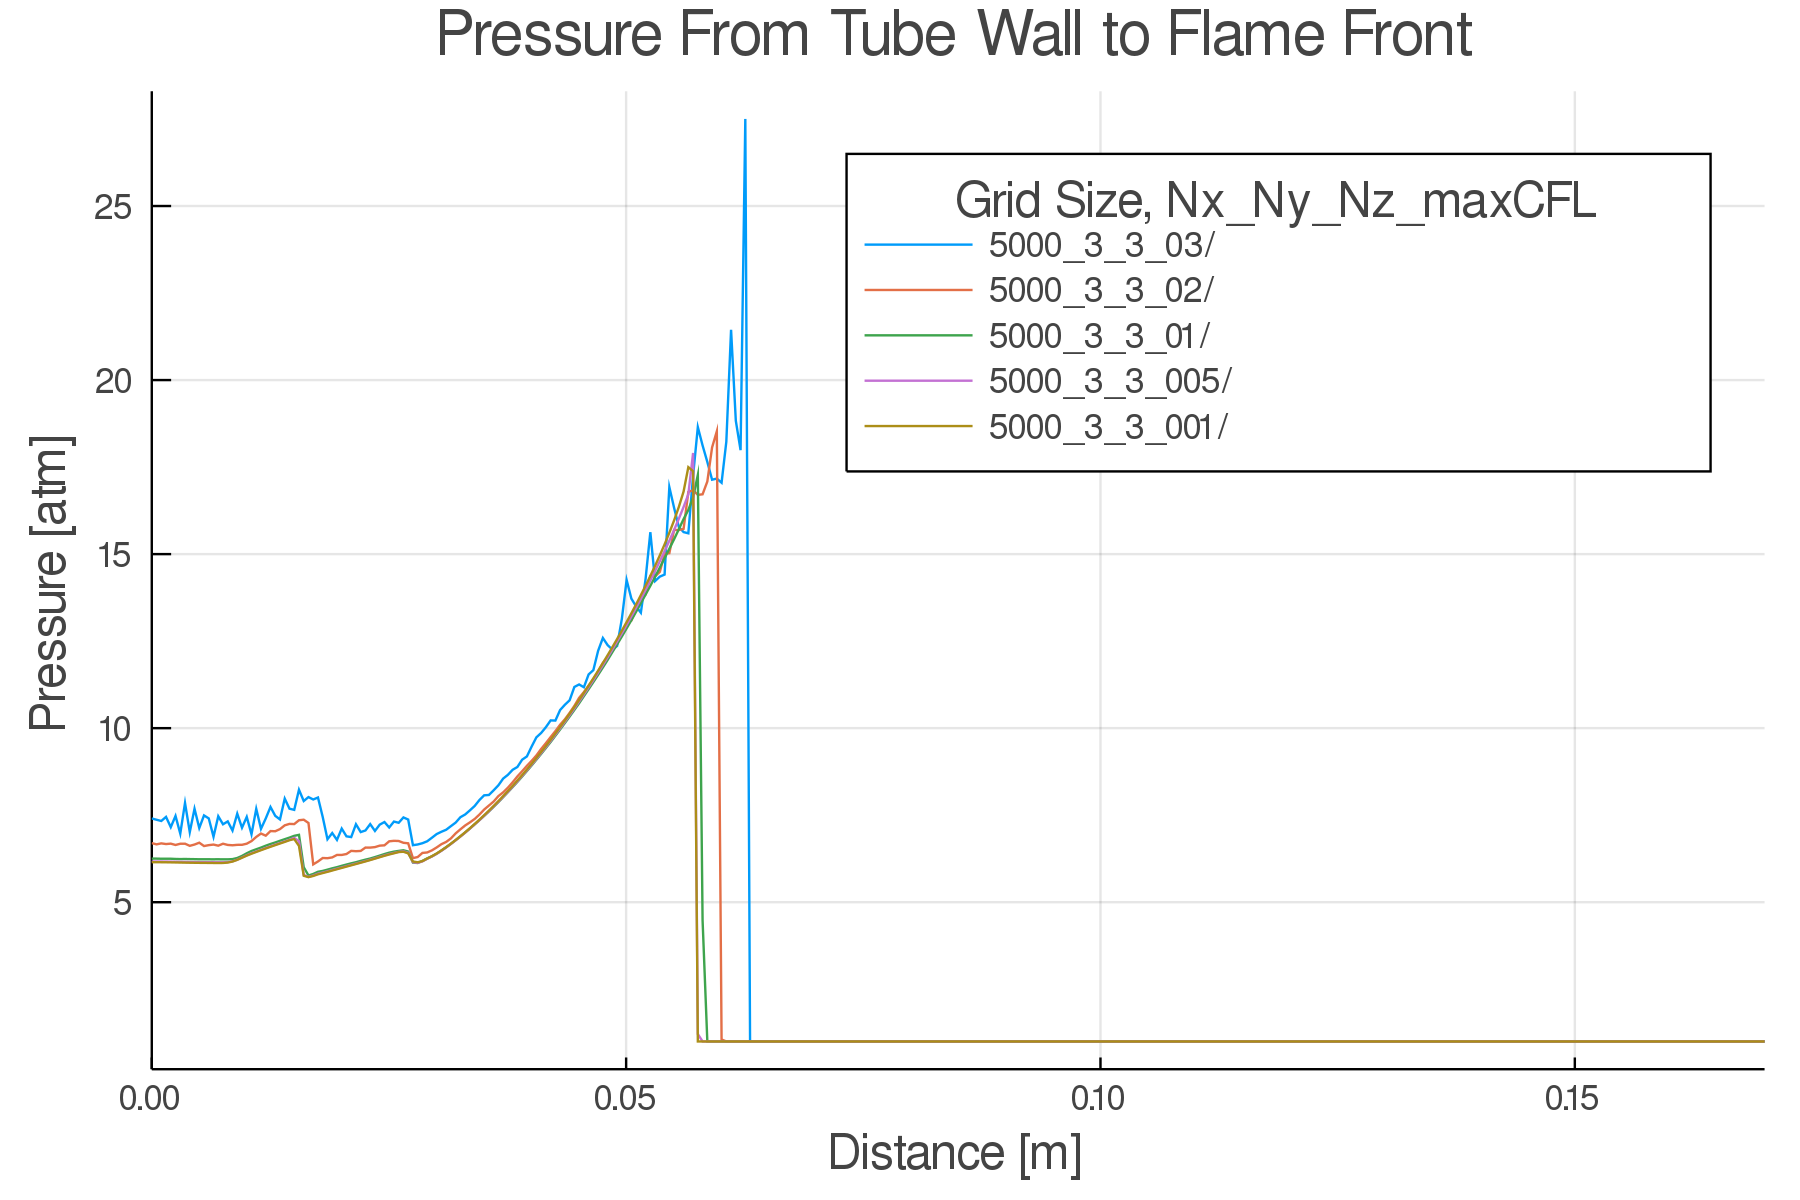
\includegraphics[width=\linewidth]{figs/cfl_test/p.png}
    \caption{Pressure distribution}
    \label{fig:cflp}
    \end{subfigure}

    \begin{subfigure}[]{\textwidth}
    \centering
    \includegraphics[width=\linewidth]{figs/cfl_test/t.png}
    \caption{Temperature distribution}
    \label{fig:cflt}
    \end{subfigure}
\end{figure}
\begin{figure}\ContinuedFloat
    \begin{subfigure}[]{\textwidth}
    \centering
    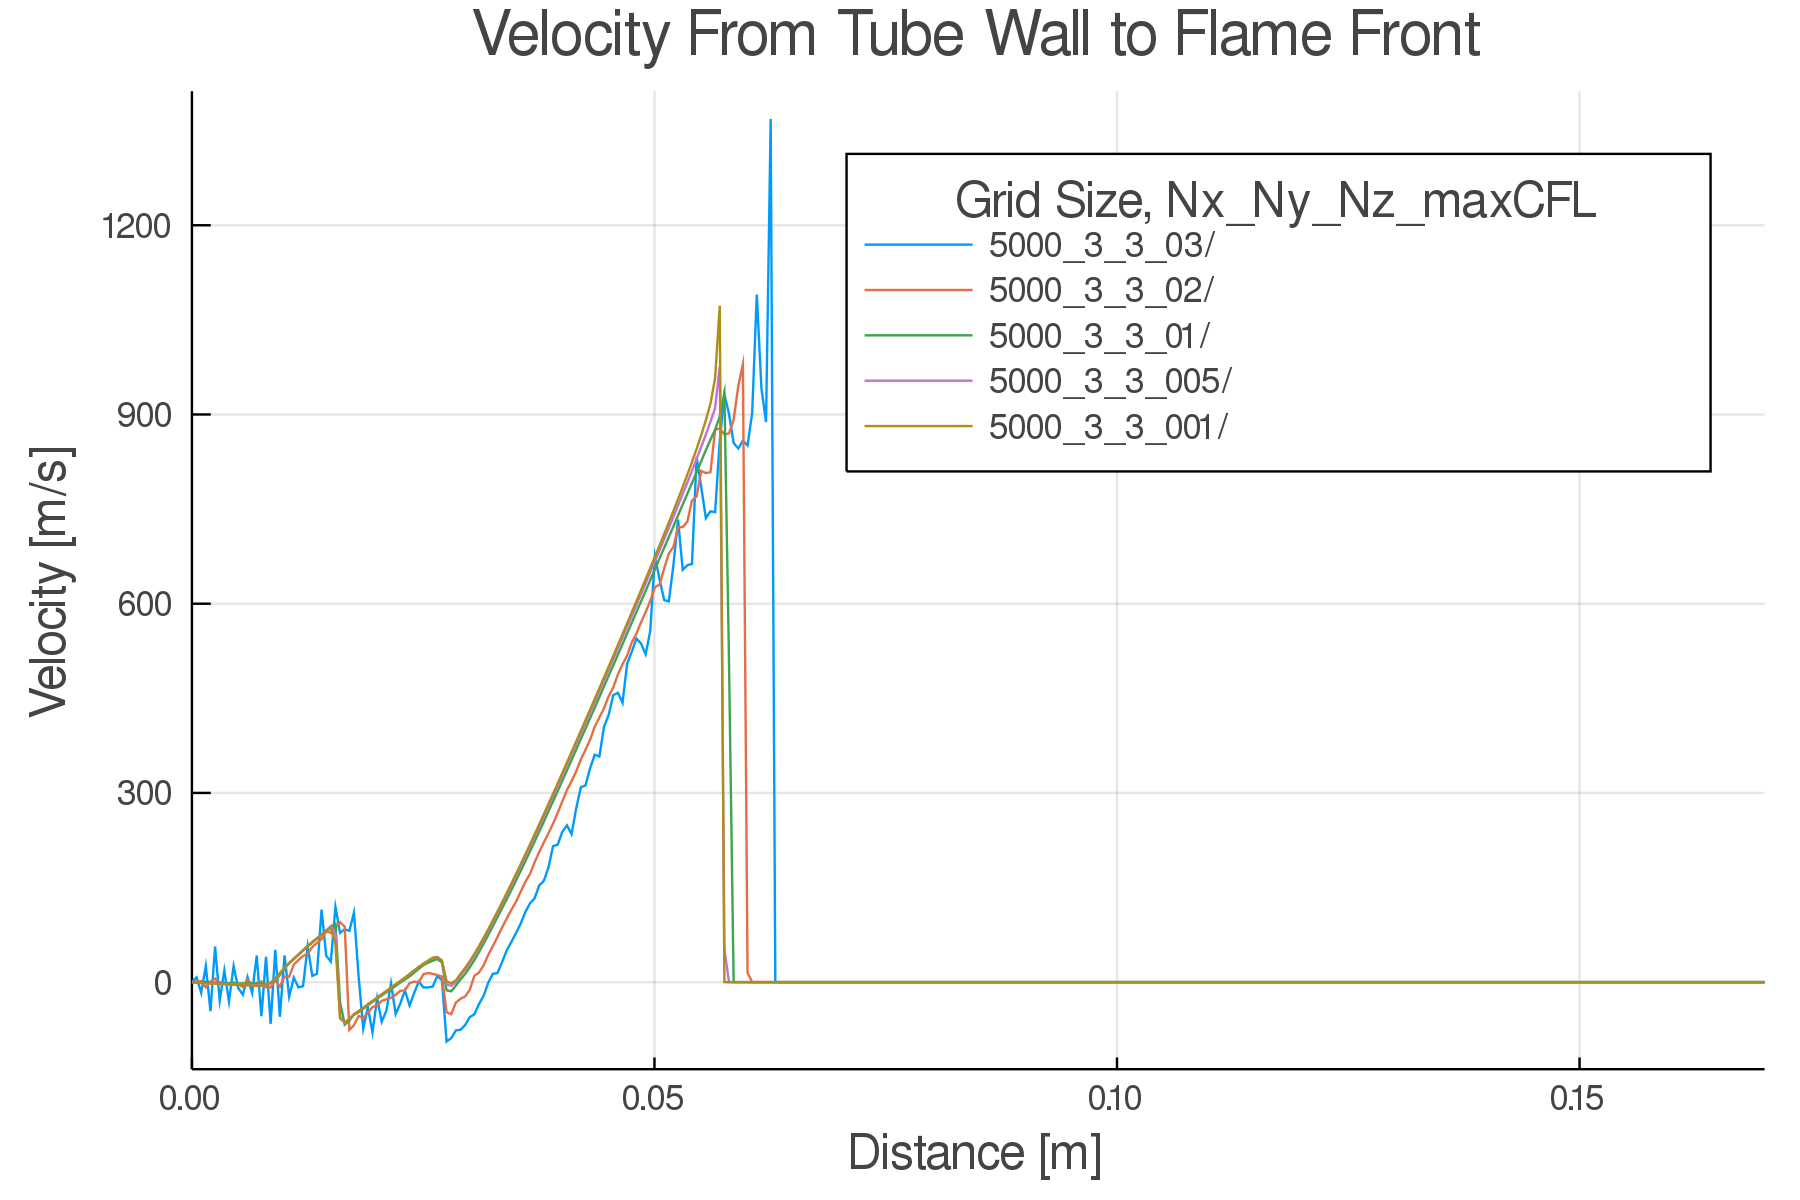
\includegraphics[width=\linewidth]{figs/cfl_test/u.png}
    \caption{Fluid velocity distribution}
    \label{fig:cflu}
    \end{subfigure}
    \caption{Max CFL sweep test}
    \label{fig:maxcfl}
\end{figure}



From Figures \ref{fig:cflp}, \ref{fig:cflt}, and \ref{fig:cflu}, it is seen that there is decreased noise in the solution as well as convergence as the time step and therefore maximum CFL is decreased. More evident in the temperature plot \ref{fig:cflt}, noise and instability is especially clear in the detonation simulations with maximum CFLs of 0.2 and 0.3. The CFL of 0.1 was decided to be acceptably converged due to a small comparative error, seen in Table \ref{tab:cflerror}. 
\begin{table}[]
\centering
\caption{Max CFL errors compared to CFL = 0.01}
\label{tab:cflerror}
\begin{tabular}{cccc}
Max CFL & Pressure Error (\%) & Temperature Error (\%) & Velocity Error (\%) \\ \hline
0.3 & 57.18 & 19.54 & 27.62 \\ 
0.2 & 5.89 & 8.72 & 8.66 \\
0.1 & 1.28 & 2.71 & 12.92 \\
0.05 & 2.34 & 1.29 & 8.96 \\
0.01 & 0 & 0 & 0 \\
\end{tabular}
\end{table}% 
\noindent Note that while the CFL of 0.2 has a smaller velocity error than the CFL of 0.1, it is a much noisier and unstable solution, so the values themselves have further uncertainty. The selection of a maximum CFL of 0.1  for detonations in OpenFOAM also matches with the work done by Ajaero\cite{ajaero}. 

Higher CFL numbers of 0.4 to 0.8 were also attempted. These were unsuccessful as the solution was extremely unstable or never converged at these CFLs. Typically, high CFL numbers cause more ringing in the solution as seen in Figure \ref{fig:maxcfl} for the CFL of 0.3. However, it is seen in this research as well as supporting reacting flow work \cite{ajaero}\cite{kim}\cite{marcantoni} lower CFL numbers are required for solution convergence. 

\section{Static Mesh Variation}
\label{sec:staticvar}
In order to determine the performance gains, accuracy, and other comparative parameters between mesh resolutions, baseline meshes must be created. These meshes must not change adaptively in the simulation in order to provide clear comparisons. Additionally, the static meshes themselves should be compared with each other to determine when mesh convergence occurs. Once a mesh resolution is determined, the AMR parameters can be tuned in an attempt to match the static mesh resolution in the small region surrounding the detonation wave. 


\subsection{One-dimensional}
\label{sec:1dstatic}

The first set of static mesh comparisons performed is between one-dimensional detonation tube simulations, seen in Figure \ref{fig:1dstatic}. These meshes only have resolution along the direction of the tube, which allows for capturing the detonation wave as simply as possible. However,  one-dimensional detonation tube simulations are not optimal for generic detonation modeling as the cellular detonation structure seen in experimental detonation modeling cannot be captured with a single dimension. The cellular detonation cells can be used to infer velocity and compare numerical simulation with experiments, so one-dimensional detonations must utilize other methods to compare with experiments or just be utilized for tuning numerical methods themselves. 

\begin{figure}[]
    \centering
    \begin{subfigure}[]{\textwidth}
        \centering
        \includegraphics[width=\textwidth]{./figs/static1d/p.png}
        \caption{Pressure plot}
    \end{subfigure}

    \begin{subfigure}[]{\textwidth}
        \centering
        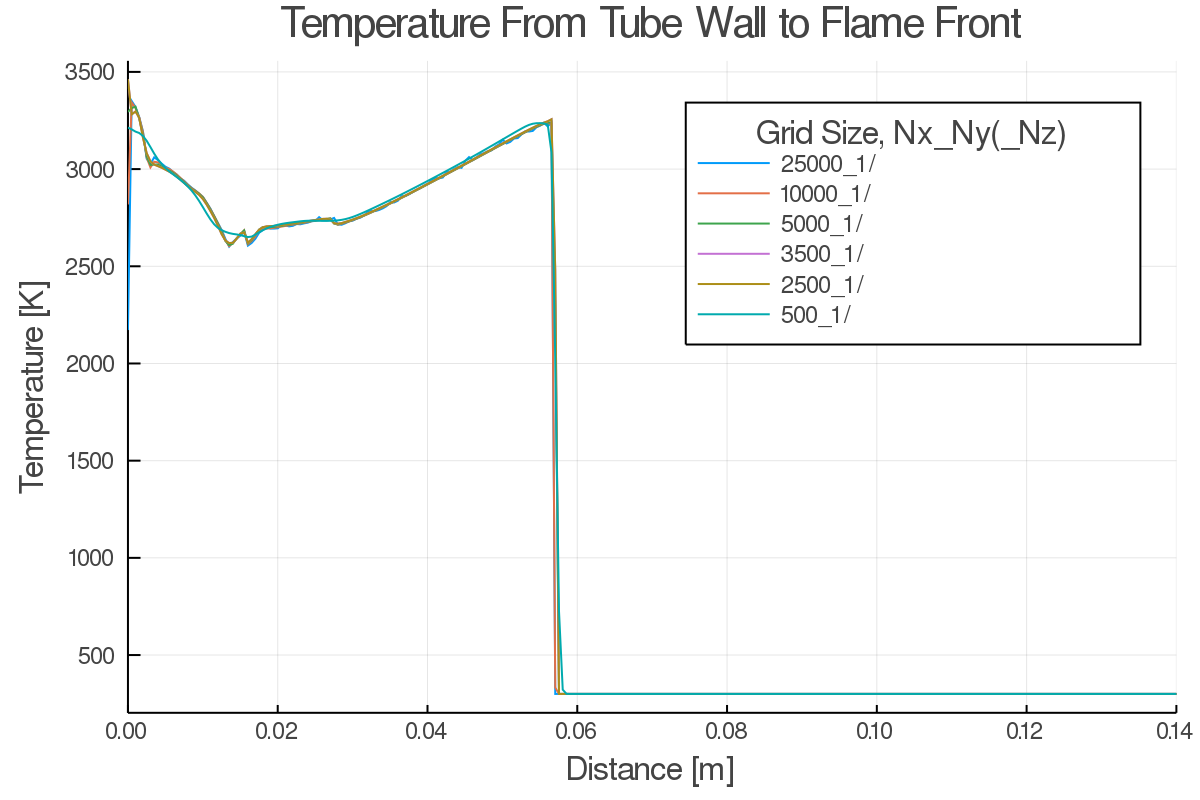
\includegraphics[width=\textwidth]{./figs/static1d/t.png}
        \caption{Temperature plot}
    \end{subfigure}

\end{figure}
\begin{figure} \ContinuedFloat
    
    \begin{subfigure}[]{\textwidth}
        \centering
        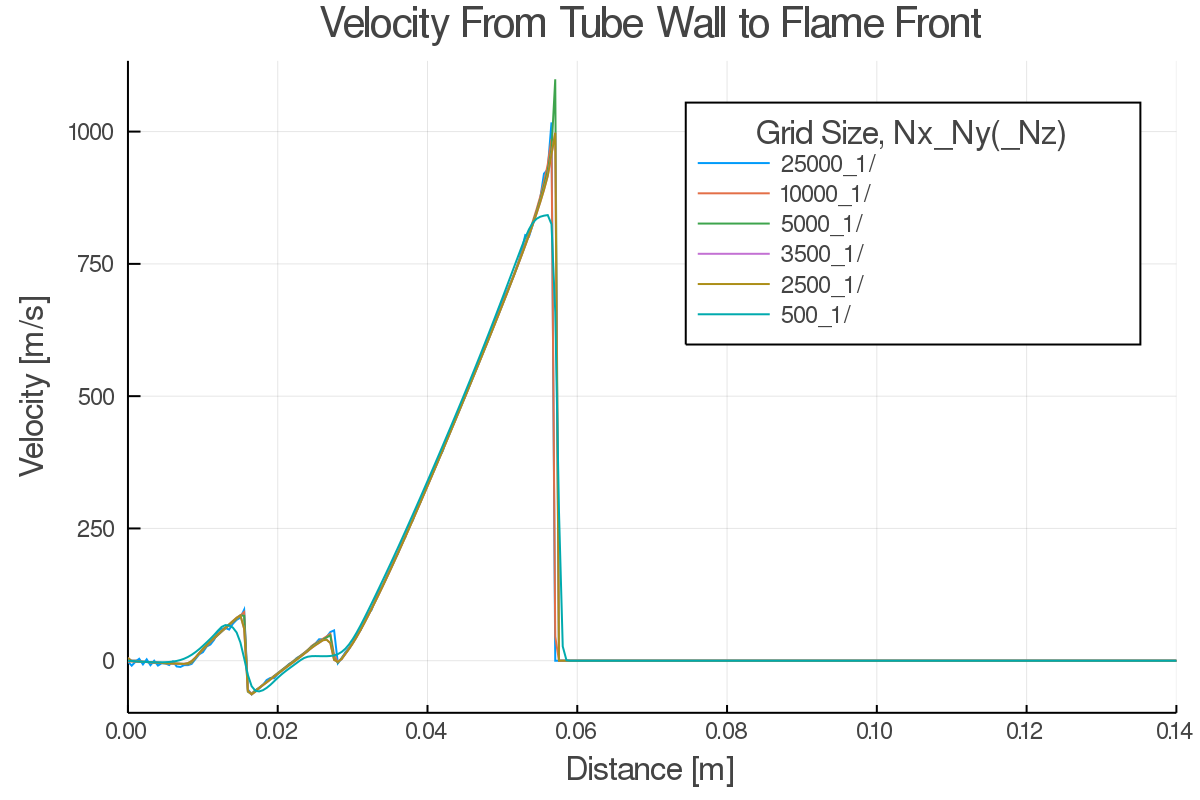
\includegraphics[width=\textwidth]{./figs/static1d/u.png}
        \caption{Fluid Velocity plot}
    \end{subfigure}

    \caption{One-dimensional static meshes used in detonation tube simulations}
    \label{fig:1dstatic}
\end{figure}

Various static one-dimensional meshes were compared and can be seen in Figure \ref{fig:1dstatic}. These one-dimensional static meshes are actually twice as long, as initially the detonation simulations were performed using a domain that was twice as long, at a half meter in length. This long mesh was unnecessarily large and computationally expensive. The mesh partition values written in the figure are divided in half to match the meshes and convention used in subsequent analysis runs, with a quarter meter long domain. We see that the 500-1-1 mesh has not converged yet to a solution, and that the 2500-1-1 mesh has converged. After this point, the difference between the meshes lies in their ability to capture finer flow effects such as detonation cells (not possible in one dimension), the transition from a singular detonation front to the combination of multiple smaller detonation fronts (also not possible in one dimension), and the increase in magnitude of the von Neumann pressure wave spike. The von Neumann spike comes from ZND detonation model theory, where Zel'dovich\cite{zeldovich}, von Neumann\cite{neumann}, and Doring\cite{doring} independently published research on a detonation model theory that utilizes an infinitesimally thin shock wave. Knowing that the spike is what changes within the converged mesh simulations allows for intelligent choices upon what sorts of AMR and static resolutions to choose both in research and engineering design. If an individual is designing a part that can withstand very fast high pressure fluctuations, then resolving the mesh up until the von Neumann spike appears will be sufficient for their design purposes. Otherwise, further mesh resolution is required in order to resolve the extremely thin pressure spike shock region. In regards to AMR, this translates to either further refinement around the spike region or just focusing refinement on the detonation wave and following region as a whole in order to resolve turbulence details or fluctuations in the field from randomization and reflected shocks. 


\subsection{Two-dimensional}
In addition to the static and dynamic one-dimensional detonation tube simulations performed, two-dimensional simulations were also run. These can be seen in Figure \ref{fig:2dstatic}. 
\begin{figure}[]
    \centering
    \begin{subfigure}[]{\textwidth}
        \centering
        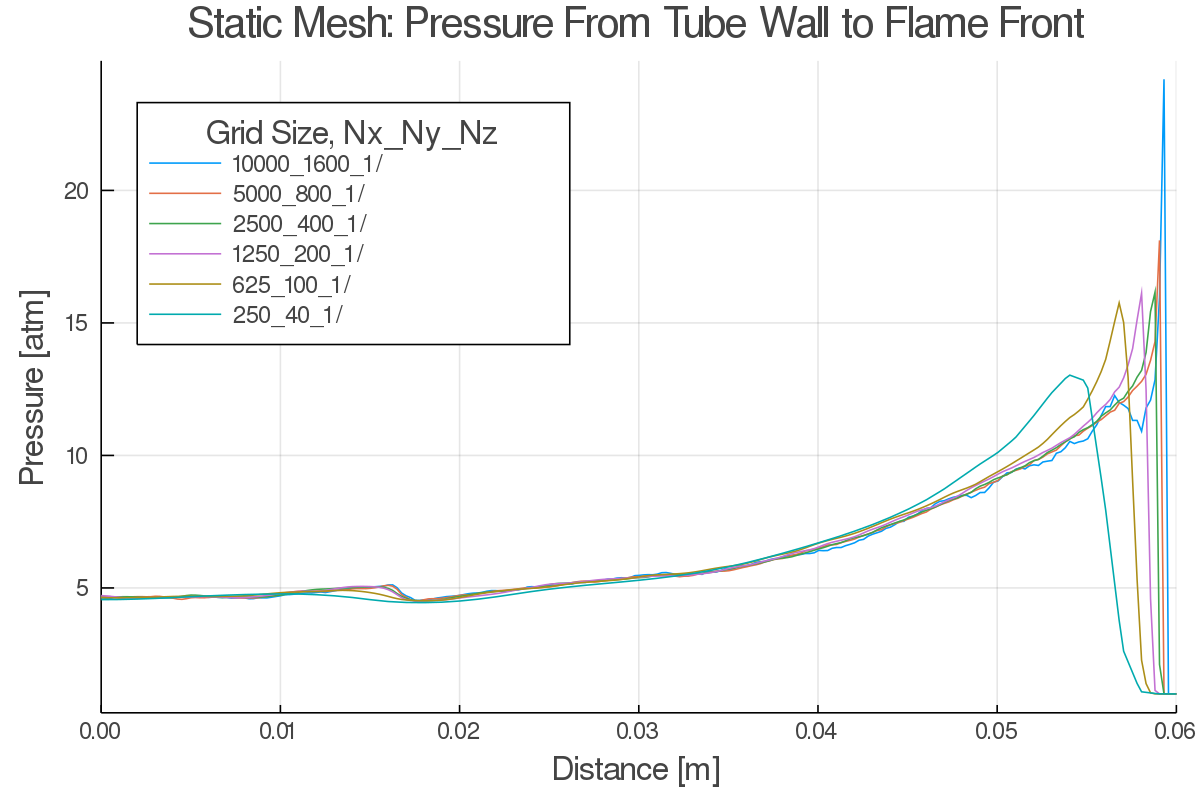
\includegraphics[width=\textwidth]{./figs/staticfigs/p.png}
        \caption{Pressure plot}
        \label{fig:2dstaticp}
    \end{subfigure}

    \begin{subfigure}[]{\textwidth}
        \centering
        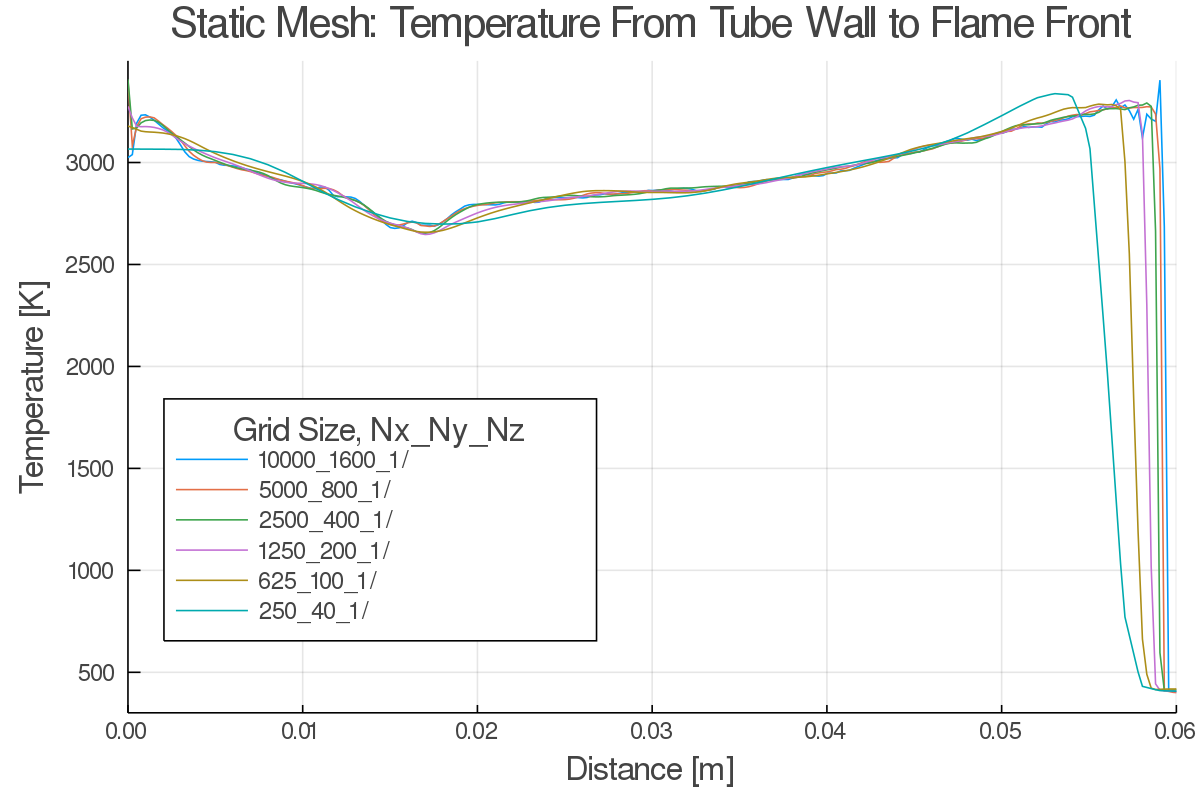
\includegraphics[width=\textwidth]{./figs/staticfigs/t.png}
        \caption{Temperature plot}
    \end{subfigure}

\end{figure}
\begin{figure} \ContinuedFloat
    
    \begin{subfigure}[]{0.95\textwidth}
        \centering
        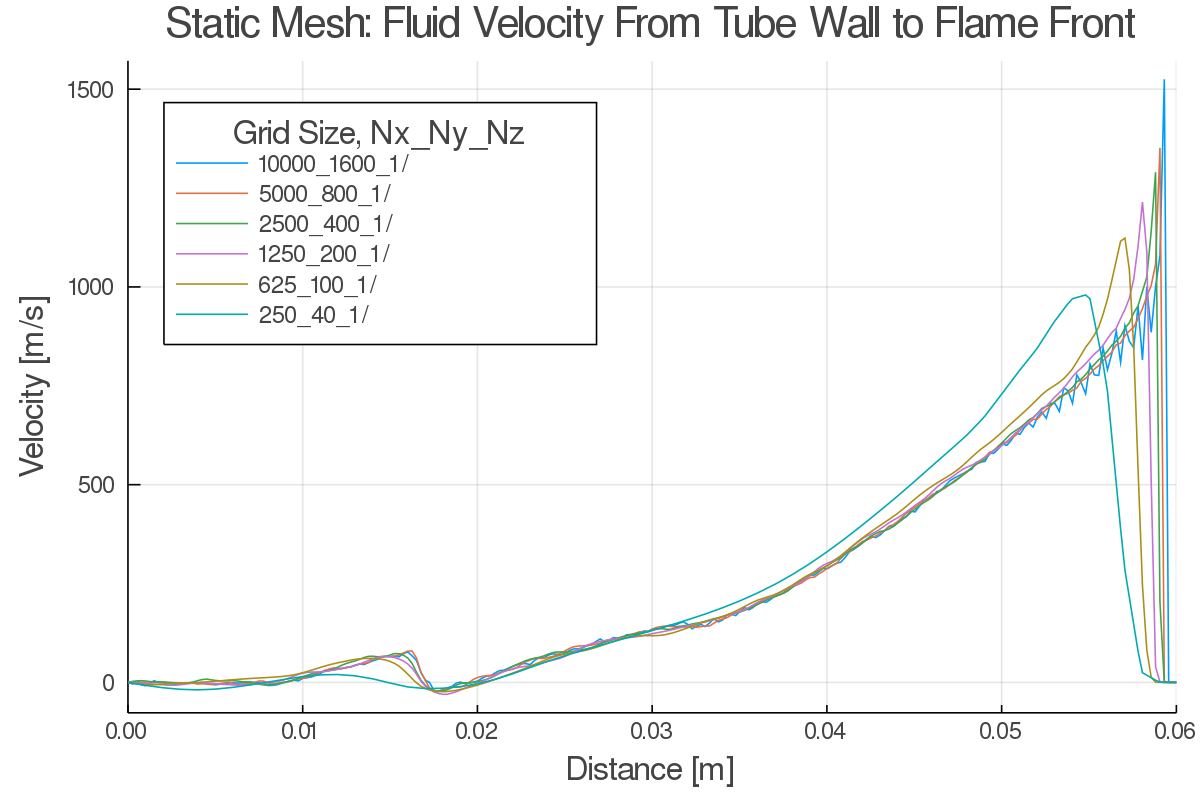
\includegraphics[width=\textwidth]{./figs/staticfigs/u.png}
        \caption{Fluid velocity plot}
        \label{fig:2dstaticu}
    \end{subfigure}

    \begin{subfigure}[]{0.95\textwidth}
        \centering
        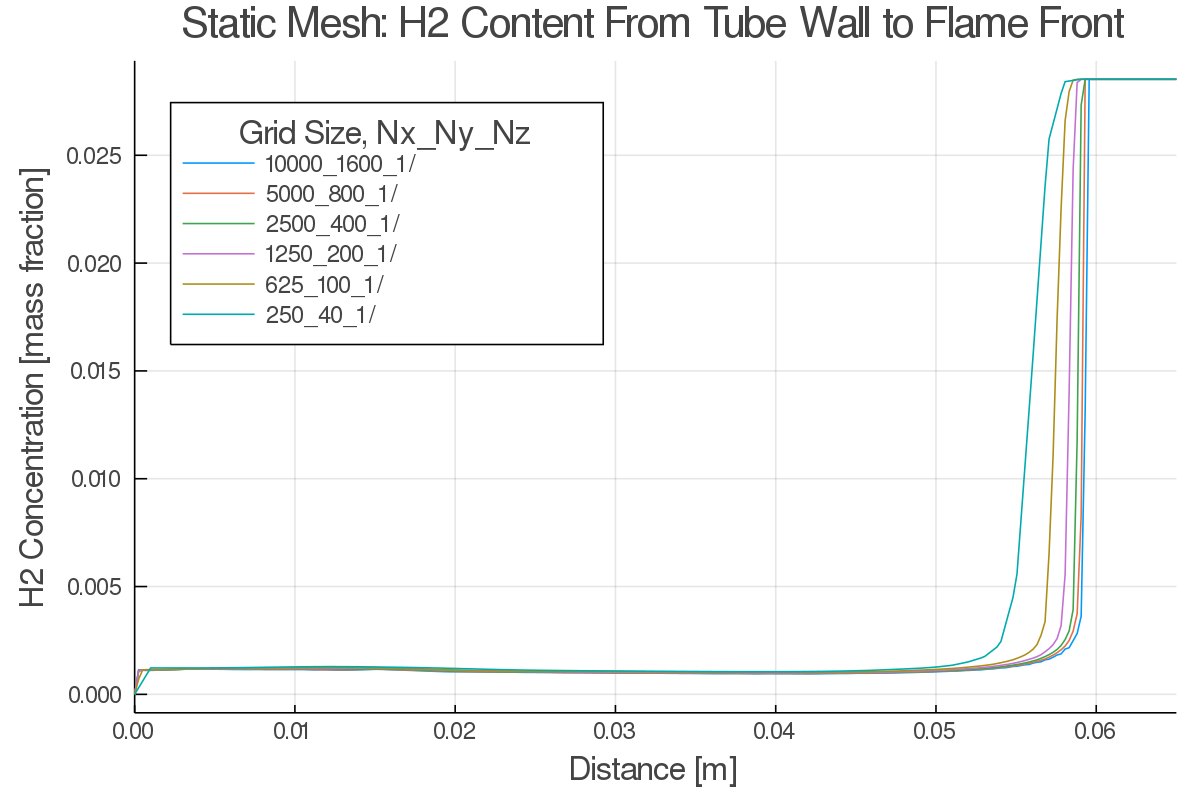
\includegraphics[width=\textwidth]{./figs/staticfigs/y.png}
        \caption{H\(_2\) mass fraction plot}
    \end{subfigure}

    \caption{Two-dimensional static meshes used in detonation tube simulations}
    \label{fig:2dstatic}
\end{figure}% 
For two-dimensional simulations, the mesh was kept square. A smaller mesh resolution than the one-dimensional simulations were used due to computational expense. The 10000-1600-1 mesh contains 16 million cells at a 25 micron physical resolution, and was computed across twenty 3.6 GHz AMD Threadripper cores at a computational time of over 150 core-hours. Note that this high mesh resolution does not have the smoothness seen in more unrefined simulation results, seen clearly in Figures \ref{fig:2dstaticp} and \ref{fig:2dstaticu}. This is due to the mesh capturing the fine shock and reaction structures described by ZND theory mentioned in Section \ref{sec:1dstatic}. The fluctuations in the temperature field begin to resolve at this resolution. 

Example surface plots for the static 2500-400-1 mesh are plotted in Figure \ref{fig:2dsurface}. 
\begin{figure}[]
    \centering
    \begin{subfigure}[]{\textwidth}
        \centering
        \includegraphics[width=\textwidth]{./figs/example_results/p.png}
        \caption{Pressure plot}
    \end{subfigure}

    \begin{subfigure}[]{\textwidth}
        \centering
        \includegraphics[width=\textwidth]{./figs/example_results/t.png}
        \caption{Temperature plot}
    \end{subfigure}

\end{figure}
\begin{figure} \ContinuedFloat
    
    \begin{subfigure}[]{\textwidth}
        \centering
        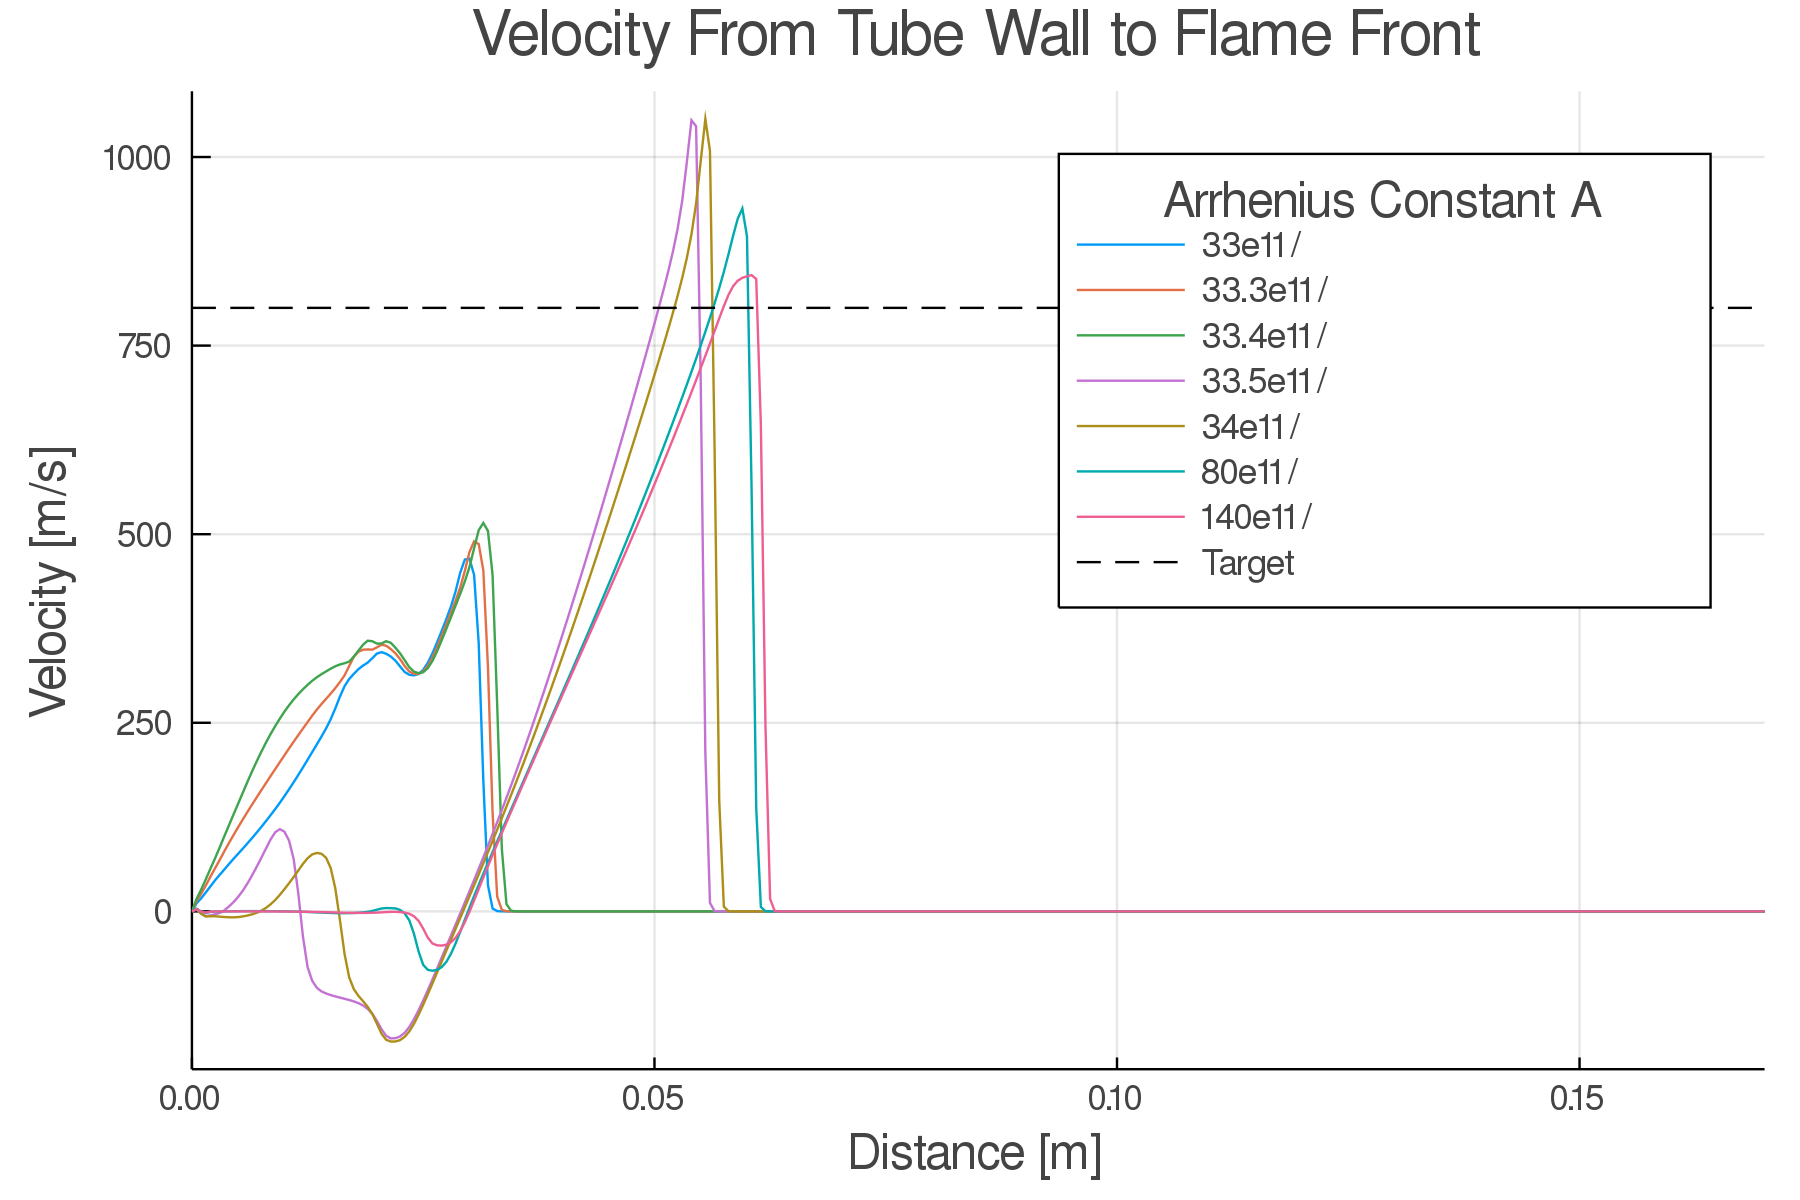
\includegraphics[width=\textwidth]{./figs/example_results/u.png}
        \caption{Fluid velocity magnitude plot}
    \end{subfigure}

    \begin{subfigure}[]{\textwidth}
        \centering
        \includegraphics[width=\textwidth]{./figs/example_results/rho.png}
        \caption{Density plot}
    \end{subfigure}

    \caption{Two-dimensional detonation wave surface plots for 2500-400-1 mesh at \(t = 3.45 \times 10^{ - 5} \) s}
    \label{fig:2dsurface}
\end{figure}% 
\noindent The plots seen in this figure represent the flow field results of a detonation wave traveling from the left wall to the right, at \(t = 3.45 \times 10^{ - 5} \) s. 





\section{Adaptive Mesh Refinement and Static Comparisons}
Since static mesh resolutions have been compared and are available for baseline comparisons, AMR was then added. As mentioned in Section \ref{sec:staticvar}, the adaptive mesh refinement parameters can be tuned to try and match the fine static mesh resolutions in important areas. Detonation waves are very thin with extremely high pressures, temperatures, and velocities within this small region. This makes them an ideal candidate for adaptive meshing. To validate the AMR routines, comparison with the baseline static meshes is required to determine how the flow field changes. The AMR settings were tweaked and changed over a range of values and compared to static meshes in order to determine if the AMR can practically replace static meshes for detonation modeling in OpenFOAM as well as attempt to characterize how each change in AMR parameter affects the solution. For the following comparison cases, it was all performed in two dimensions. This allows for the AMR to start delivering noticeable performance gains as cell counts can often quickly increase into the millions. 

The primary variable used to track when the AMR should be applied was the normalized gradient of pressure, \( ||\nabla(p)||\). Detonations  and shock waves will have very large pressure gradients, so this is a logical selection. By normalizing this quantity, the values selected for the bounds are always consistent across any similar simulation and the setup is easier. Other variables can also be selected for refinement tracking variables, such as pressure, temperature, and velocity. The reasons that these were not selected as primary tracked variables was due to the rest of the flow field. Pressure itself could change significantly between different simulations, so normalized pressure is probably a better choice. Even if normalized pressure is chosen, a portion of the field can remain at high pressure (i.e. in the burning region after the detonation). The pressure gradient waveform is much sharper and thinner than pressure, so this provides a better small region for the AMR to focus on. Temperature is fairly consistent across the products and even increases back towards the detonation initiation region, so tracking temperature itself around the wave only would be very difficult. Velocity and normalized velocity may be appropriate, but only for initiated detonations as the ignition region has no flow field velocity and therefore the important initial refinement of the flow field as the detonation wave is forming will not occur due to the lack of velocity before the reactants ignite and detonate. Exploration in combining parameters together to track or different tracking parameters altogether is a topic for further research. 


\subsection{AMR Refine Level Comparisons}
One of the more important parameters to test is the number of times the adaptive meshing routines refine each cell, or the refinement level. A 125-20-1 base mesh was used to test each refinement level using the normalized pressure gradient as the tracked variable with three buffer layers. The results, taken at \(3\times 10^{ - 5}\) s, are plotted in Figure \ref{fig:amr_refinelevels}.
\begin{figure}[]
    \centering
    \begin{subfigure}[]{\textwidth}
        \centering
        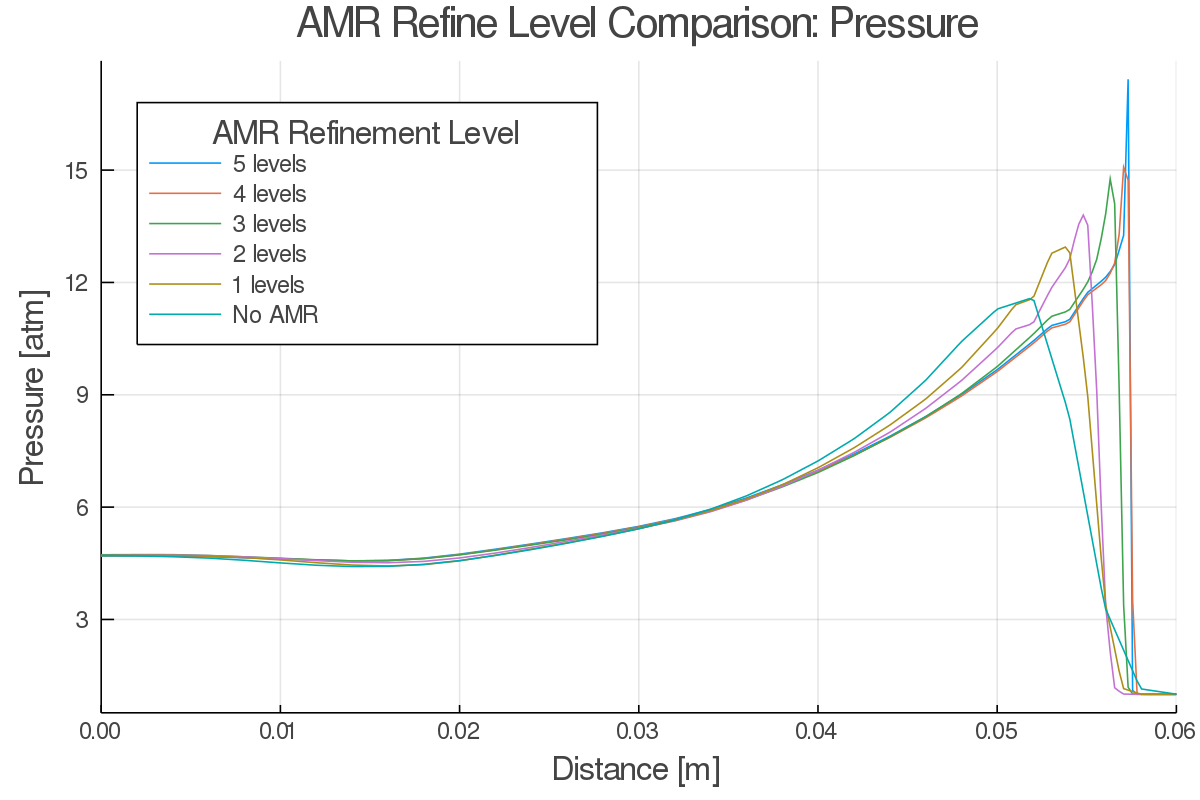
\includegraphics[width=\textwidth]{./figs/amrfigs/amr_refinelevels/p.png}
        \caption{Pressure plot}
    \end{subfigure}

    \centering
    \begin{subfigure}[]{\textwidth}
        \centering
        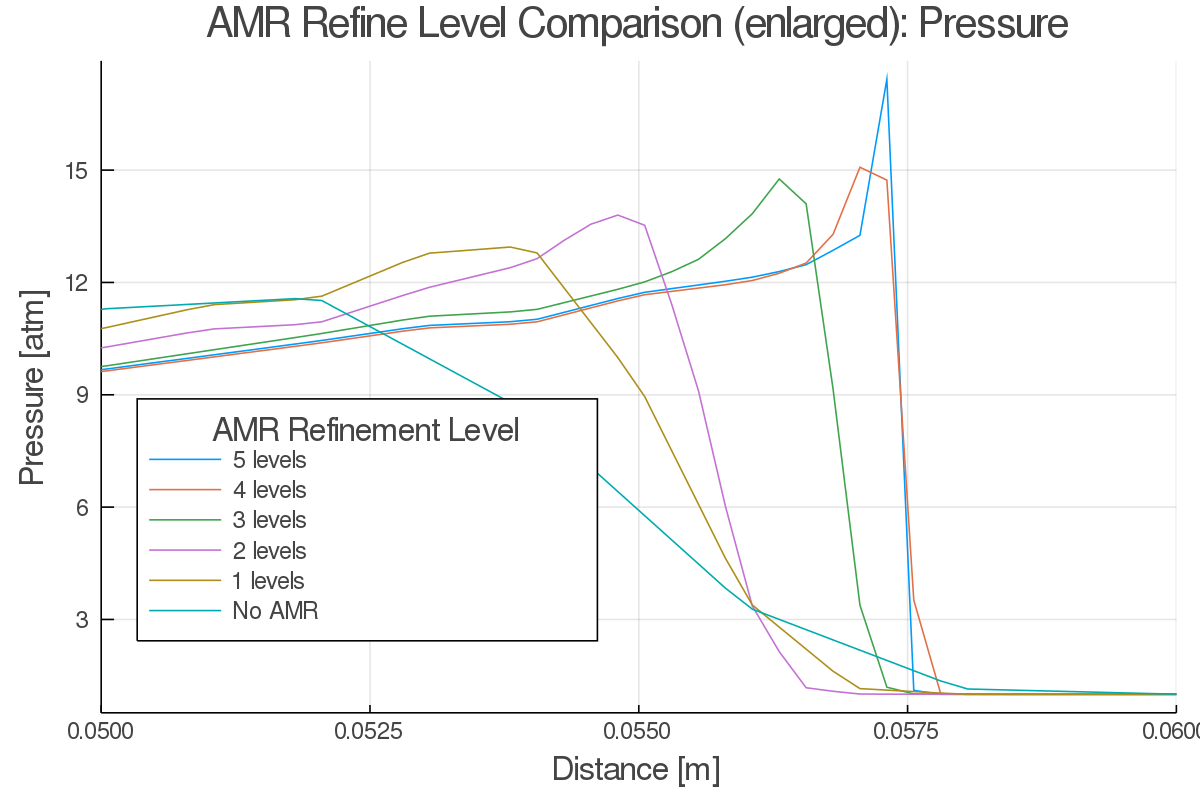
\includegraphics[width=\textwidth]{./figs/amrfigs/amr_refinelevels/pe.png}
        \caption{Pressure plot, enlarged}
    \end{subfigure}

\end{figure}
\begin{figure} \ContinuedFloat

    \centering
    \begin{subfigure}[]{\textwidth}
        \centering
        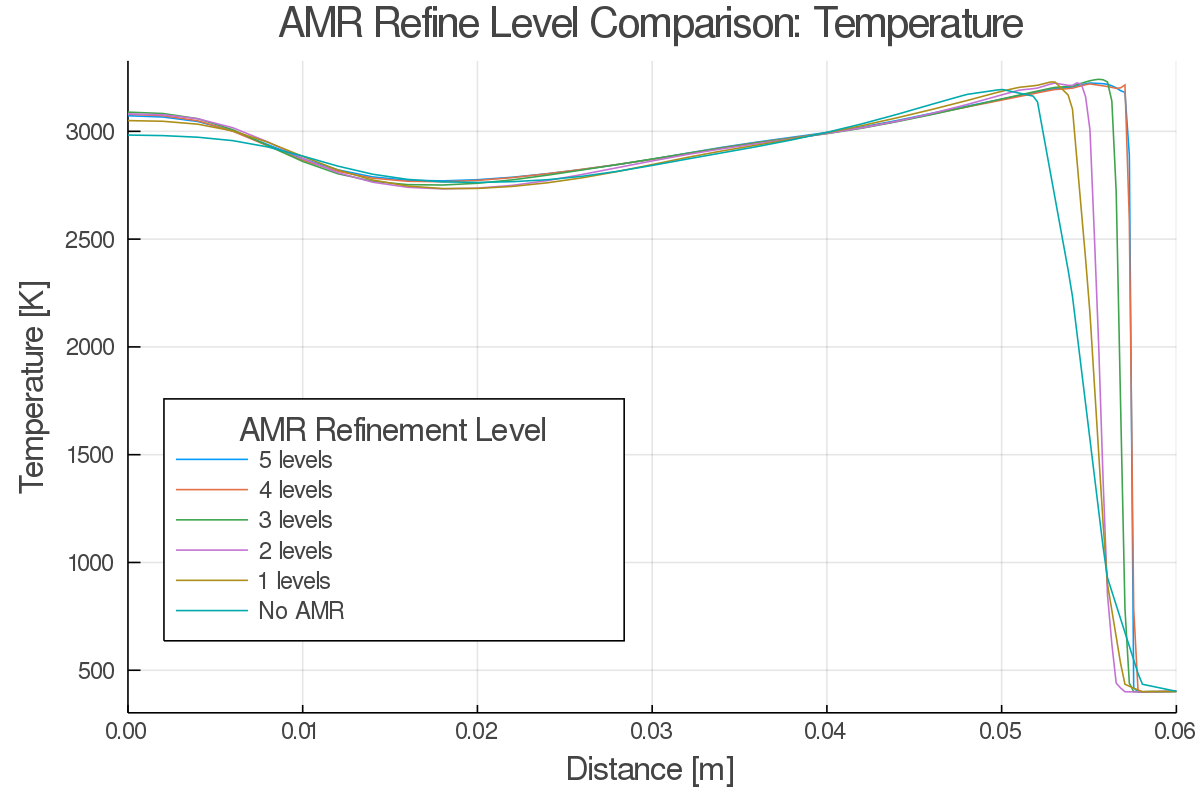
\includegraphics[width=\textwidth]{./figs/amrfigs/amr_refinelevels/t.png}
        \caption{Temperature plot}
    \end{subfigure}

    \centering
    \begin{subfigure}[]{\textwidth}
        \centering
        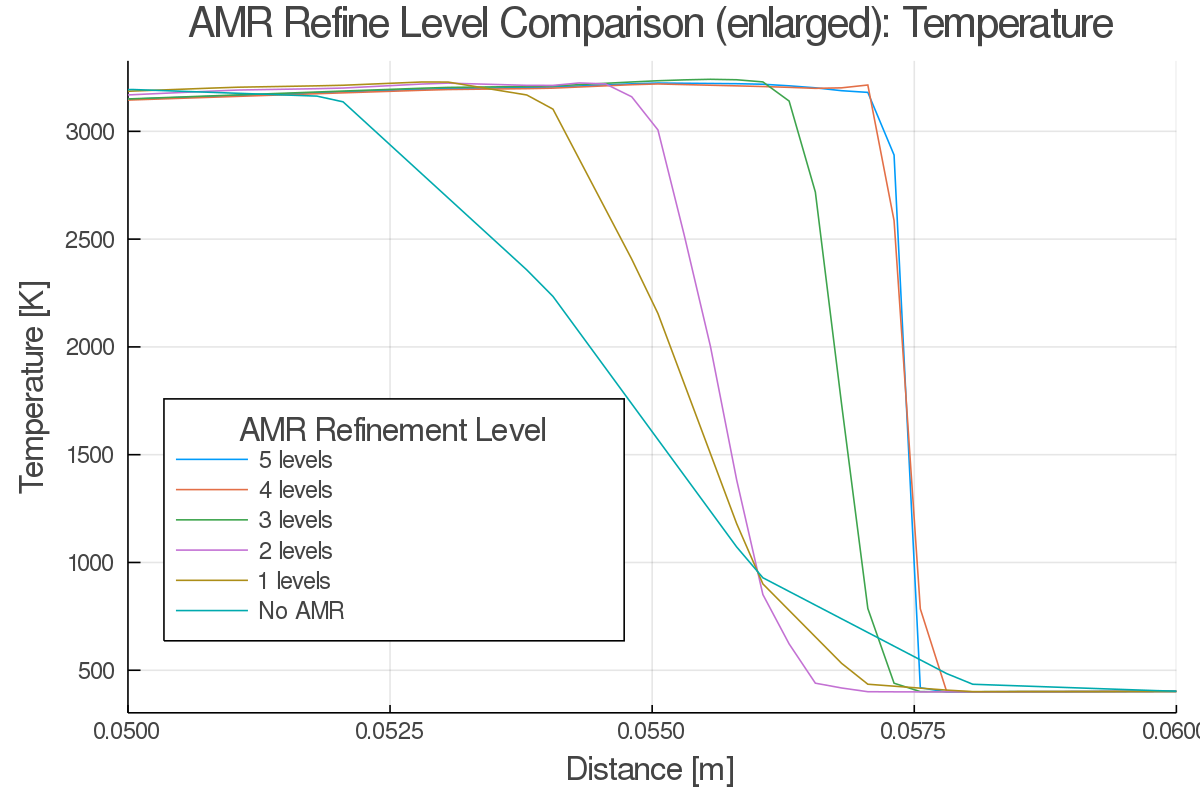
\includegraphics[width=\textwidth]{./figs/amrfigs/amr_refinelevels/te.png}
        \caption{Temperature plot, enlarged}
    \end{subfigure}

\end{figure}
\begin{figure} \ContinuedFloat
    
    \centering
    \begin{subfigure}[]{\textwidth}
        \centering
        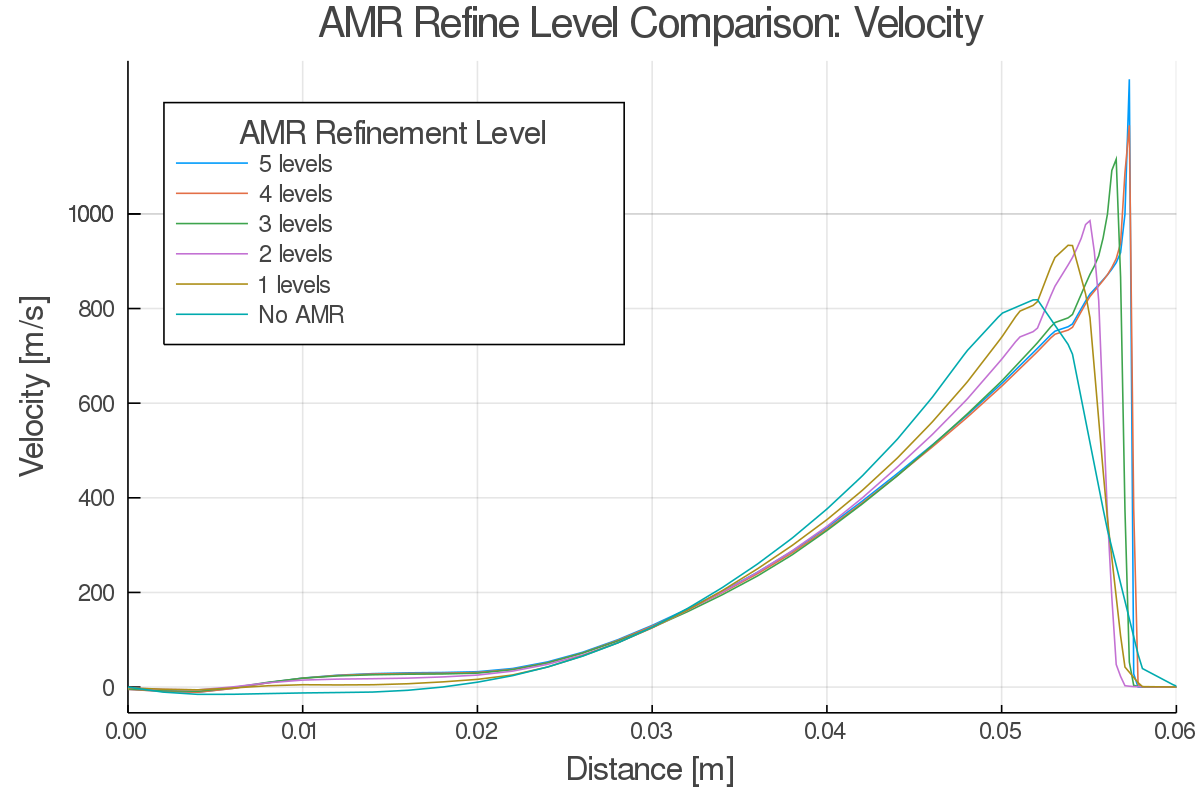
\includegraphics[width=0.9\textwidth]{./figs/amrfigs/amr_refinelevels/u.png}
        \caption{Fluid velocity plot}
    \end{subfigure}

    \centering
    \begin{subfigure}[]{\textwidth}
        \centering
        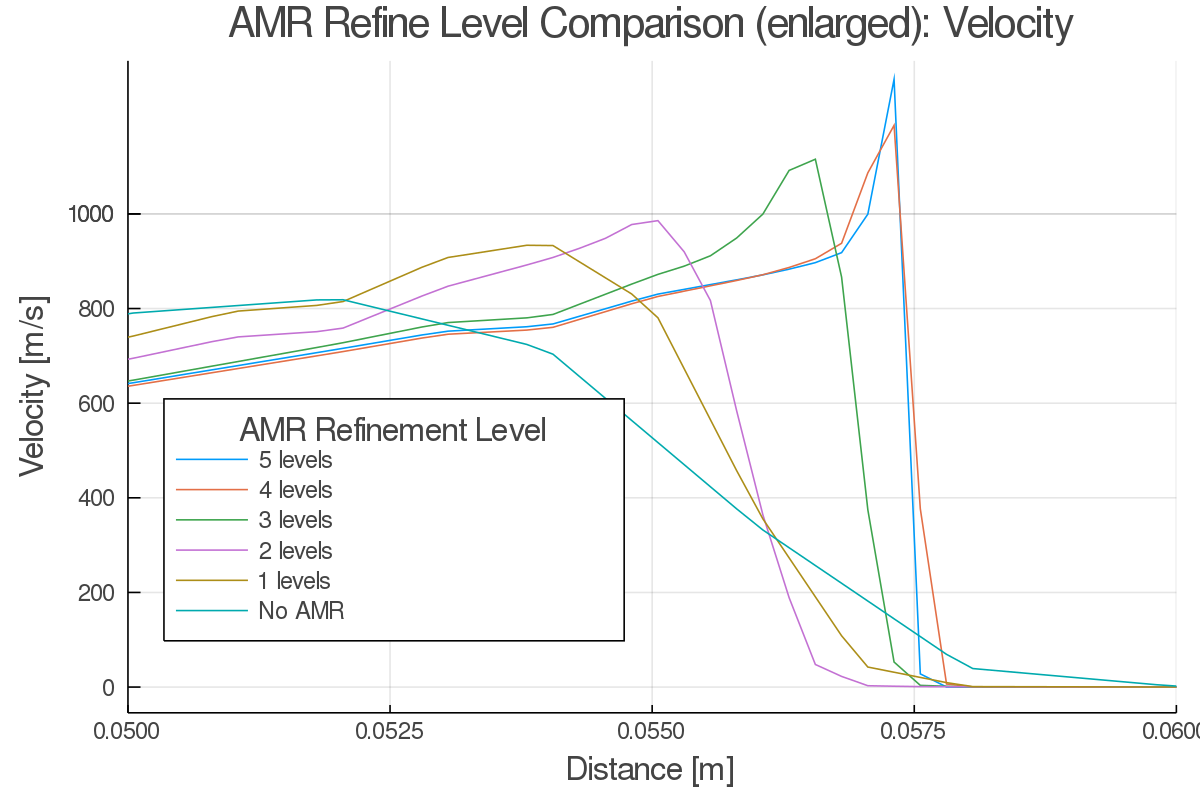
\includegraphics[width=0.9\textwidth]{./figs/amrfigs/amr_refinelevels/ue.png}
        \caption{Fluid velocity plot, enlarged}
    \end{subfigure}

    \caption{Two-dimensional detonation wave AMR results for a 125-20-1 base mesh with 3 buffer layers, tracking \( ||\nabla(p)||\) between 0.2 and 1 at 3e-5 s, sweeping refinement levels}
    \label{fig:amr_refinelevels}
\end{figure}% 
\noindent As expected, as the refinement level increases, so does the accuracy of the detonation wave. For this particular base mesh, it can be seen that the solution starts to converge around 4 levels of refinement and after the von Neumann pressure spike begins to resolve. For different base resolutions and simulation setups, this may change. It can also be seen that each increase in refinement level brings the solution roughly as close to a potential ``perfect'' static mesh resolution by half the previous x-distance, with the increase in pressure solution being exponential due to the resolving of the von Neumann spike. Further refinement levels are similarly as expensive, being exponential in cell growth, seen in Table \ref{tab:amr_refinelevels}. The exponential cell growth was also reflected in the time the simulations took to complete. The level 5 refinement has nearly the same peak pressure value as the 5000-800-1 simulation, with a slight spatial offset and 3,771,393 fewer cells. Further tweaking with tracked variable bounds as well as buffer layers may bring the detonation wave closer to that static mesh simulation. After 4 and more refinement levels (e.g. 4000-640-1 mesh) the von Neumann spike begins to resolve, which agrees with the static 2D mesh results. 


\begin{table}[h]
\centering
\caption{Cells for each refinement level for the 125-20-1 simulation at \(t = 3\times 10^{ - 5} s\) in Figure \ref{fig:amr_refinelevels}}
\label{tab:amr_refinelevels}
\begin{tabular}{cc}
Refinement Level & Cells \\ \hline
5 & 228,607 \\ 
4 & 54,678 \\ 
3 & 13,028 \\ 
2 & 5,300 \\
1 & 2,920 \\
None & 2500 \\
\end{tabular}
\end{table}

\subsection{AMR Buffer Layer Comparisons}
Within the AMR settings, different numbers of buffer layers between the refinement layer and the rest of the flow can be set. A 250-40-1 base mesh was set, with 3 refinement levels tracking the normalized pressure gradient \( ||\nabla(p)||\) from 0.2 to 1. Different number of buffer layers were tested and plotted at \(t = 3 \times 10^{ - 5}\) s in Figure \ref{fig:amr_bufflayers}. 
\begin{figure}[]
    \centering
    \begin{subfigure}[]{\textwidth}
        \centering
        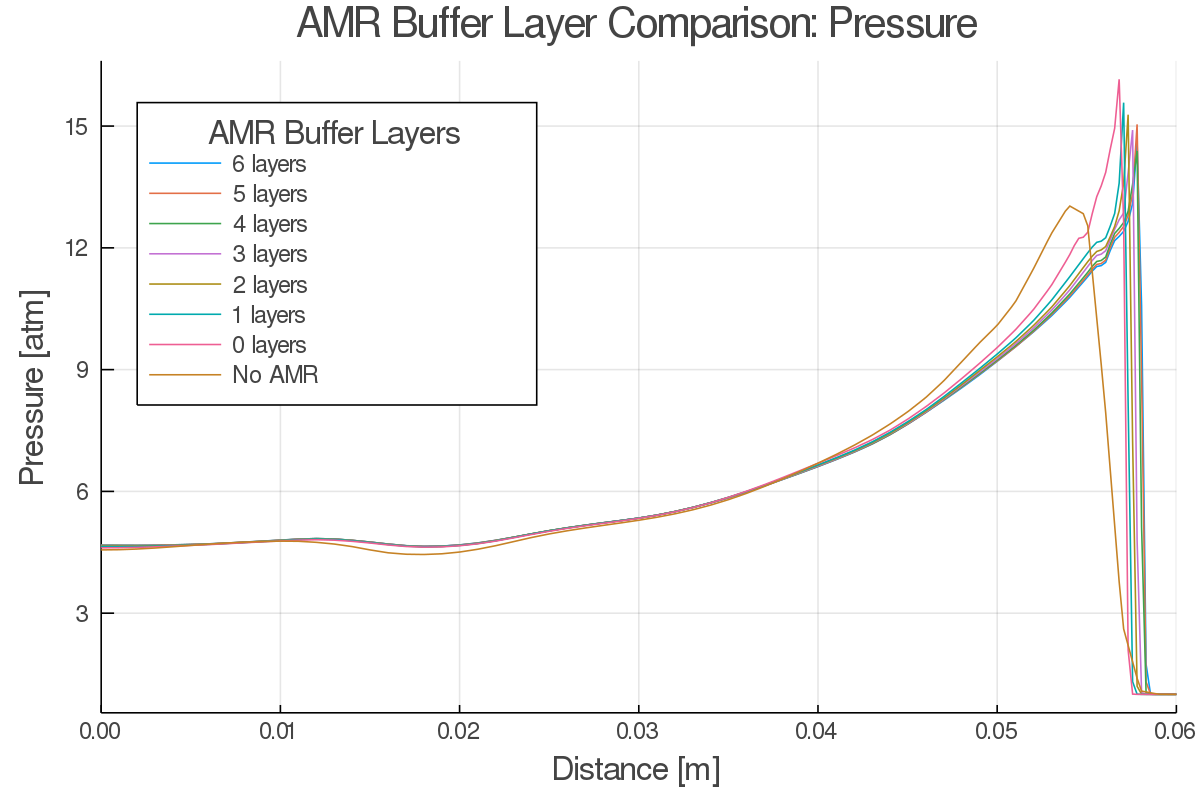
\includegraphics[width=\textwidth]{./figs/amrfigs/amr_bufflayers/p.png}
        \caption{Pressure plot}
    \end{subfigure}

    \centering
    \begin{subfigure}[]{\textwidth}
        \centering
        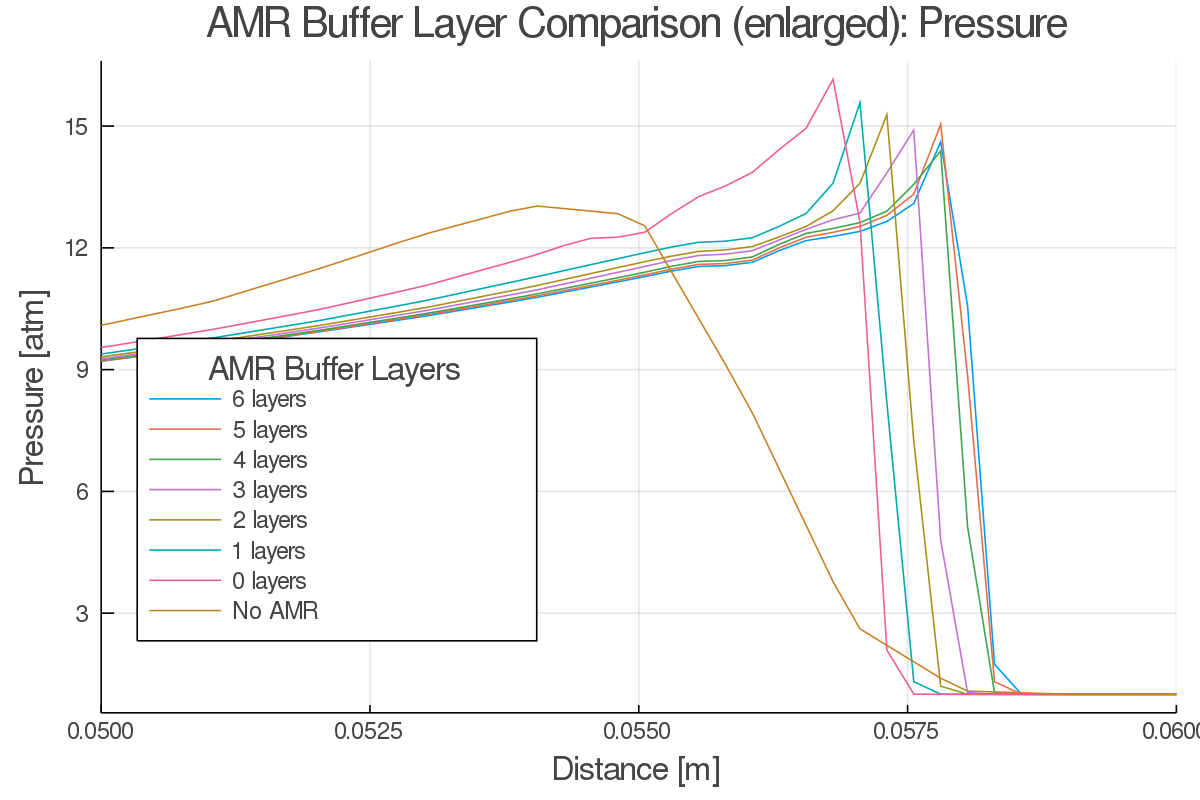
\includegraphics[width=\textwidth]{./figs/amrfigs/amr_bufflayers/pe.png}
        \caption{Pressure plot, enlarged}
    \end{subfigure}

\end{figure}
\begin{figure} \ContinuedFloat

    \centering
    \begin{subfigure}[]{\textwidth}
        \centering
        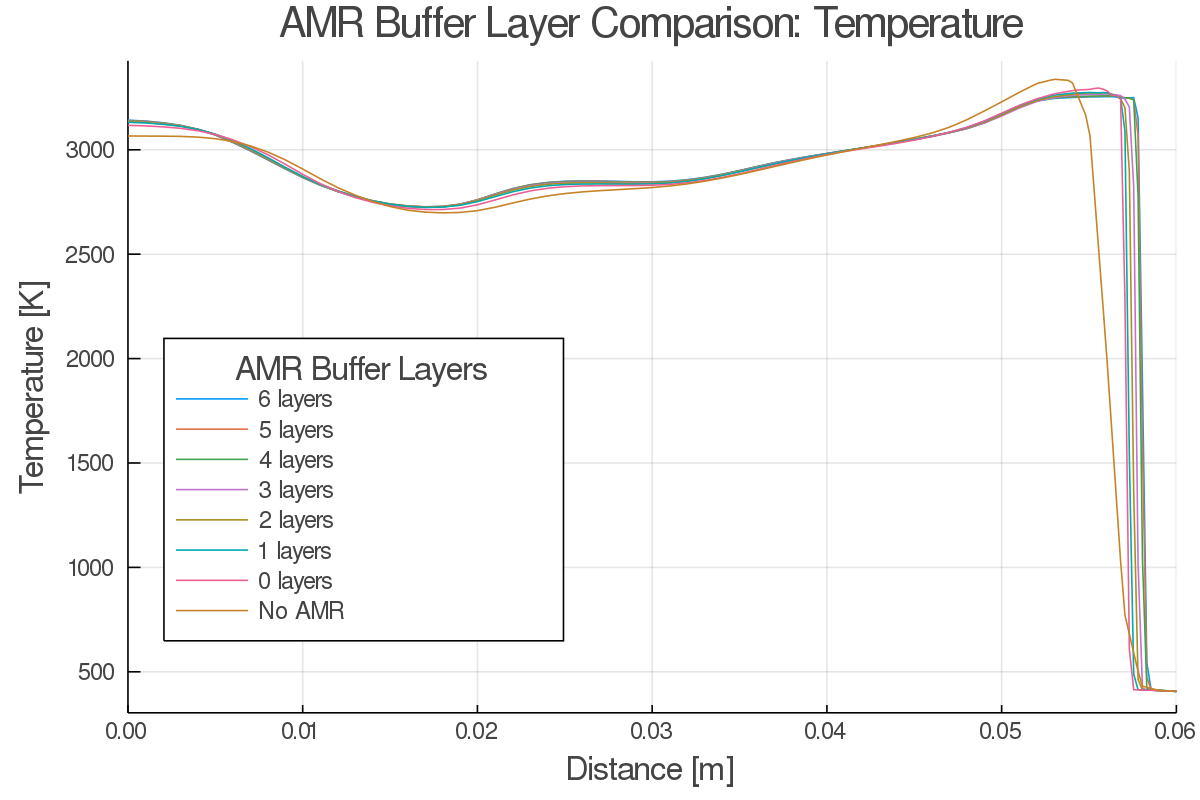
\includegraphics[width=\textwidth]{./figs/amrfigs/amr_bufflayers/t.png}
        \caption{Temperature plot}
    \end{subfigure}

    \centering
    \begin{subfigure}[]{\textwidth}
        \centering
        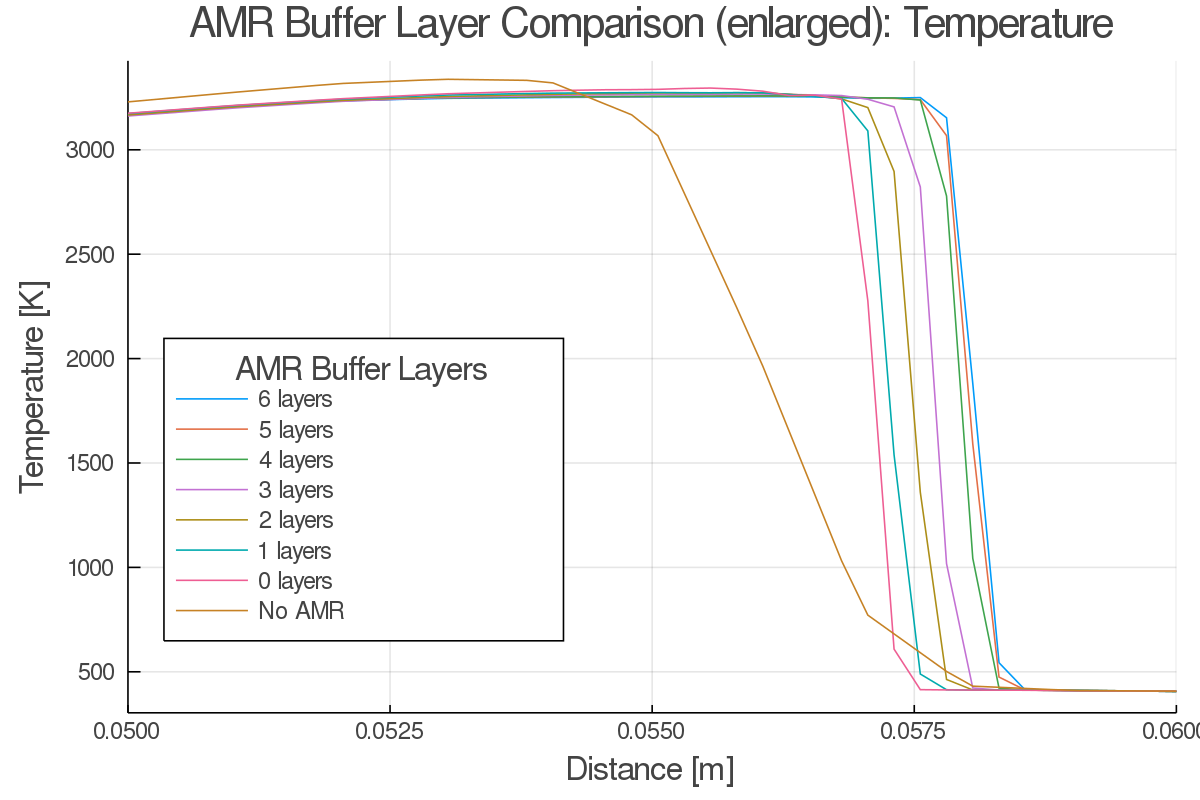
\includegraphics[width=\textwidth]{./figs/amrfigs/amr_bufflayers/te.png}
        \caption{Temperature plot, enlarged}
    \end{subfigure}

\end{figure}
\begin{figure} \ContinuedFloat
    
    \centering
    \begin{subfigure}[]{\textwidth}
        \centering
        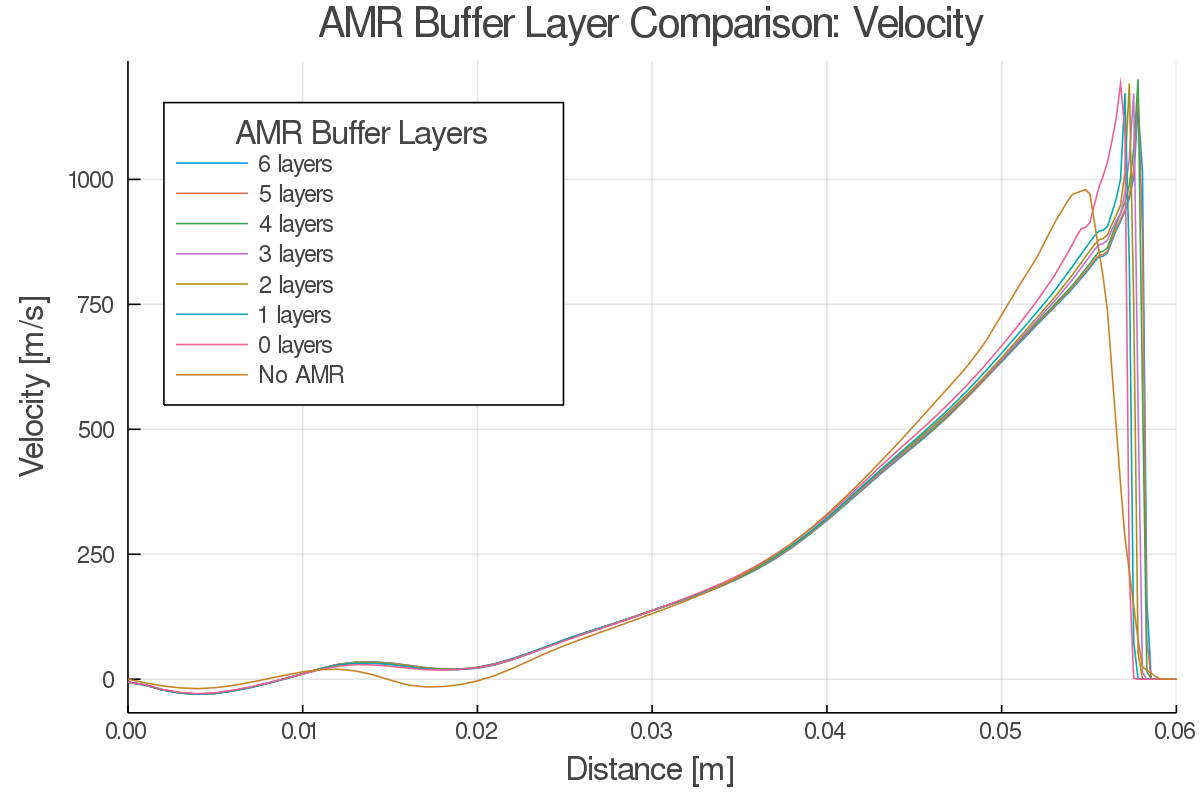
\includegraphics[width=0.9\textwidth]{./figs/amrfigs/amr_bufflayers/u.png}
        \caption{Fluid velocity plot}
    \end{subfigure}

    \centering
    \begin{subfigure}[]{\textwidth}
        \centering
        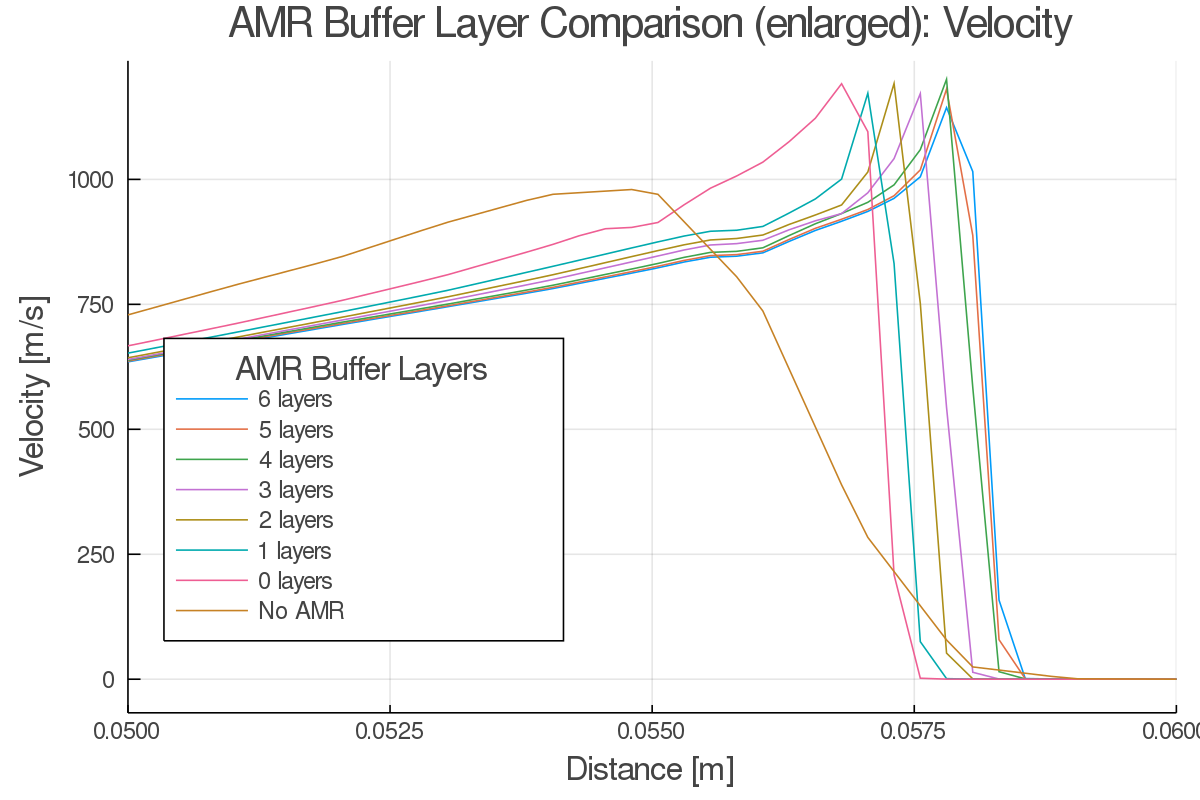
\includegraphics[width=0.9\textwidth]{./figs/amrfigs/amr_bufflayers/ue.png}
        \caption{Fluid velocity plot, enlarged}
    \end{subfigure}

    \caption{Two-dimensional detonation wave AMR results for a 250-40-1 base mesh with 3 refinement levels, tracking \( ||\nabla(p)||\) between 0.2 and 1 at 3e-5 s, sweeping buffer layers}
    \label{fig:amr_bufflayers}
\end{figure}% 
\noindent From the figure, it can be seen that the pressure solution generally decreases and the wave propagates further right, around 0.2 mm per layer, as more buffer layers are added. When 4 buffer layers are reached, the buffer layers have ``converged'' with their overall affect on the solution. Due to this, we can conclude that for PDEs and detonation tube simulations 4 buffer layers are sufficient and significant improvements in solution accuracy are not worth the increased cell count which could be used for additional refinement layers or an increased AMR refinement range. That said, the subjective timing of adding additional buffer layers was not as significant as additional refinement levels. The maximum temperature and velocity seen do not change beyond using AMR or not, but the location of the detonation wave does as with the rest of the solution variables. When a user is attempting to move the AMR-simulated detonation wave closer to static results while tuning AMR parameters, adding additional buffer layers up to 5 layers will move the AMR-simulated detonation wave close to static simulation results at minimal additional cost. Table \ref{tab:amr_bufflayers} displays the cell counts for each additional AMR buffer layer for the simulations tested in Figure \ref{fig:amr_bufflayers}. For each additional buffer layer, there is roughly a linear increase in cells, which tracks with the time the simulations took to complete. 

\begin{table}[h]
\centering
\caption{Cells for each refinement level for the 250-40-1 simulation at \(t = 3\times 10^{ - 5} s\) in Figure \ref{fig:amr_bufflayers}}
\label{tab:amr_bufflayers}
\begin{tabular}{cc}
Buffer Layers & Cells \\ \hline
6 & 37,405 \\ 
5 & 34,353 \\
4 & 32,960 \\
3 & 37,678 \\
2 & 16,173 \\
1 & 10,840 \\
None & 10,000 \\
\end{tabular}
\end{table}


\subsection{AMR Normalized Pressure Gradient Refinement Range Comparisons}
In addition to the levels of refinement and buffer layers, the actual range in which the normalized pressure gradient is refined over can be altered. The upper bound of the normalized pressure gradient tracking variable was kept at 1, with the lower refinement bound and the unrefine bound kept identical and swept across a range of values. As a reminder, if the normalized pressure gradient is between 1 and the lower bound, adaptive meshing will be active within the cell. If the value is lower than the unrefinement bound, unrefinement of the cell until the base resolution will occur. This was plotted at \(3\times 10^{ - 5}\) s in Figure \ref{fig:amr_refinebounds}. 
\begin{figure}[]
    \centering
    \begin{subfigure}[]{\textwidth}
        \centering
        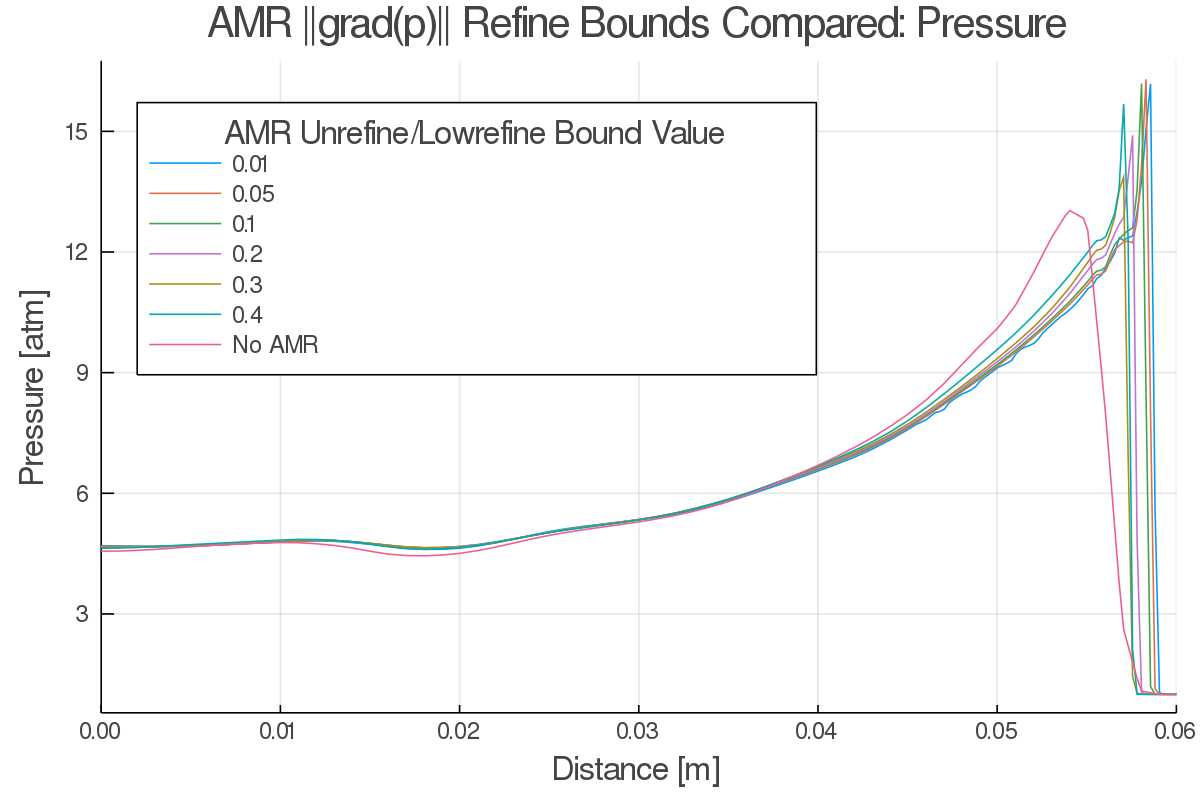
\includegraphics[width=\textwidth]{./figs/amrfigs/amr_refinebounds/p.png}
        \caption{Pressure plot}
    \end{subfigure}

    \centering
    \begin{subfigure}[]{\textwidth}
        \centering
        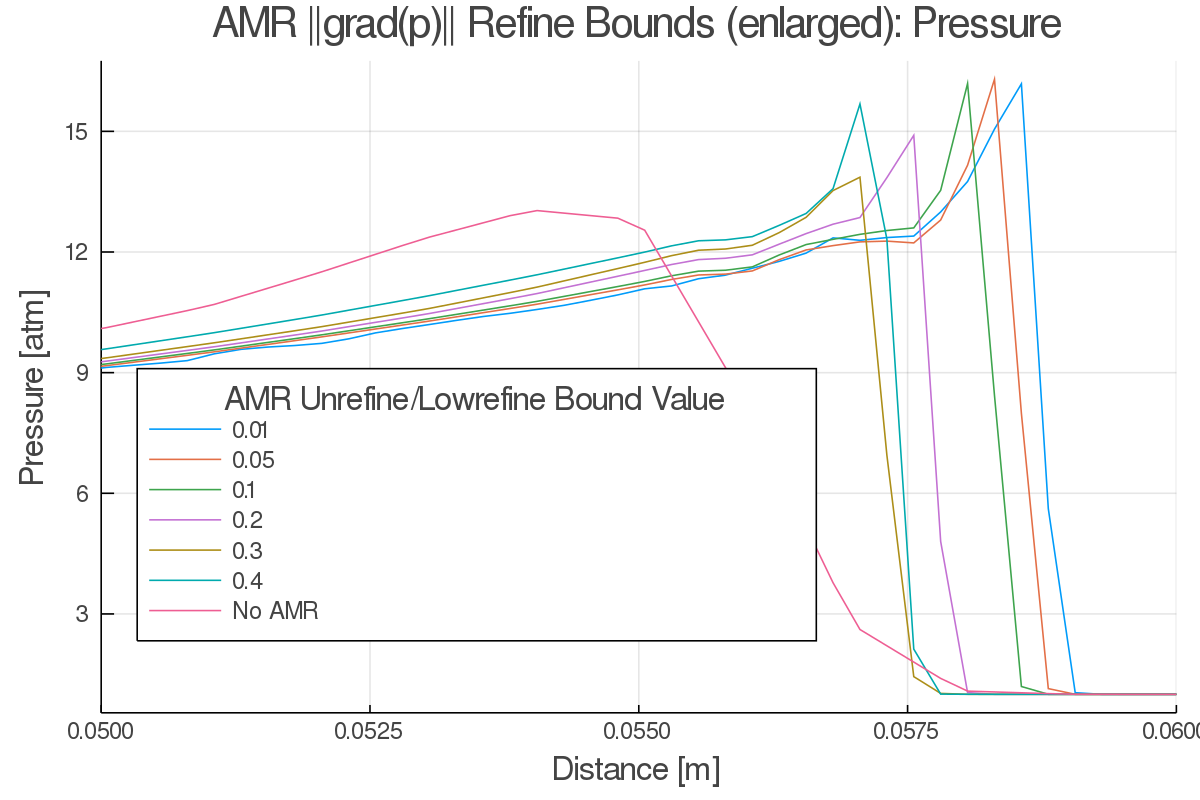
\includegraphics[width=\textwidth]{./figs/amrfigs/amr_refinebounds/pe.png}
        \caption{Pressure plot, enlarged}
    \end{subfigure}

\end{figure}
\begin{figure} \ContinuedFloat

    \centering
    \begin{subfigure}[]{\textwidth}
        \centering
        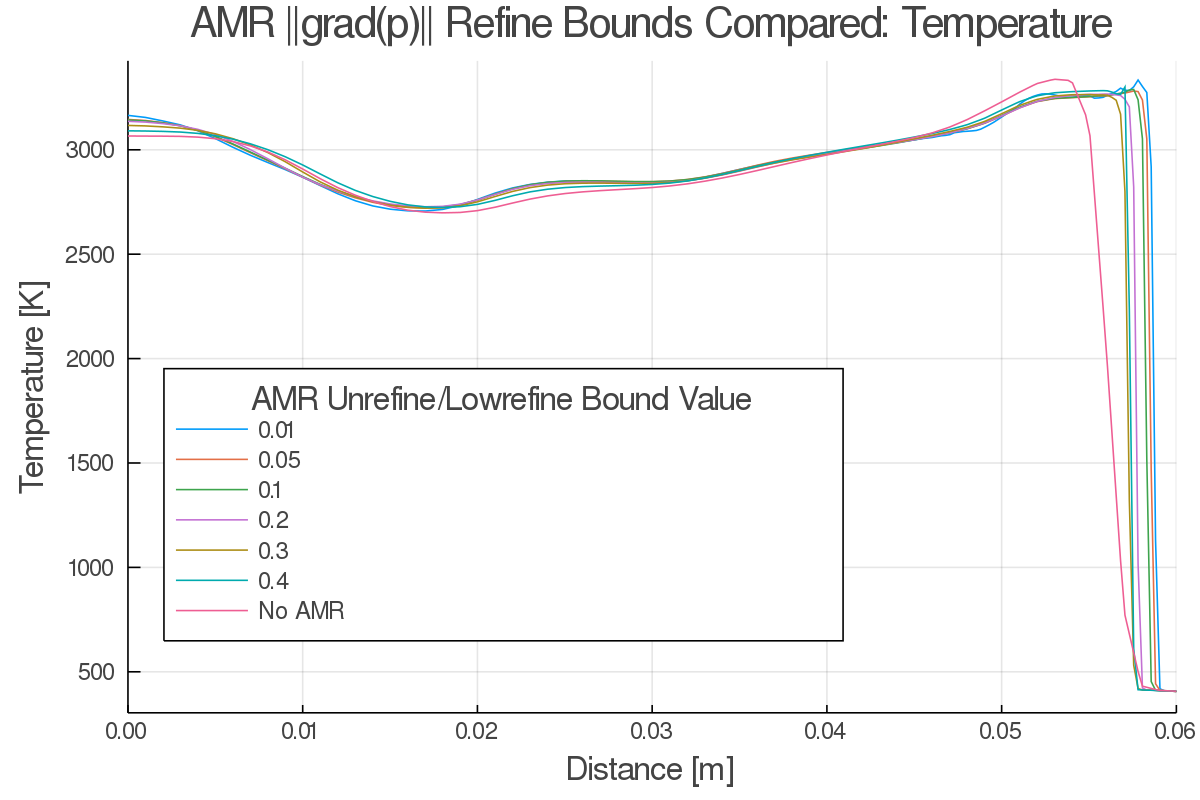
\includegraphics[width=\textwidth]{./figs/amrfigs/amr_refinebounds/t.png}
        \caption{Temperature plot}
    \end{subfigure}

    \centering
    \begin{subfigure}[]{\textwidth}
        \centering
        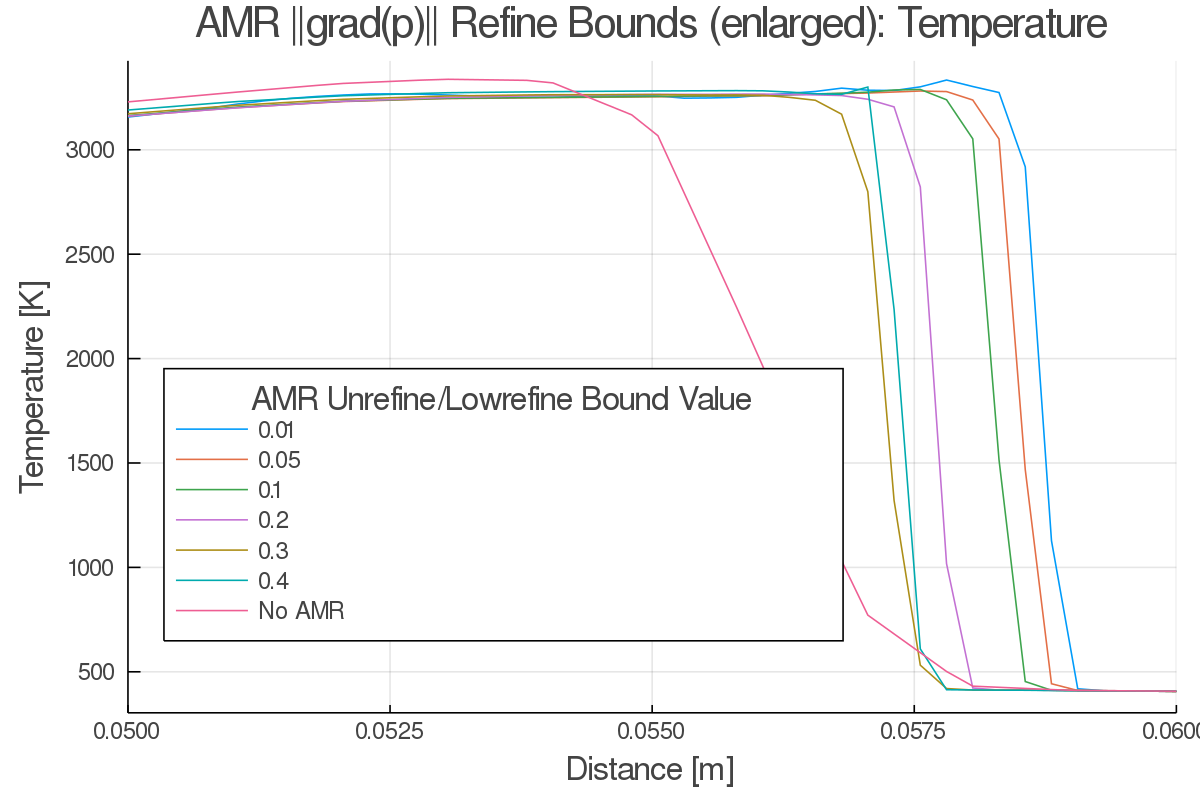
\includegraphics[width=\textwidth]{./figs/amrfigs/amr_refinebounds/te.png}
        \caption{Temperature plot, enlarged}
    \end{subfigure}

\end{figure}
\begin{figure} \ContinuedFloat
    
    \centering
    \begin{subfigure}[]{\textwidth}
        \centering
        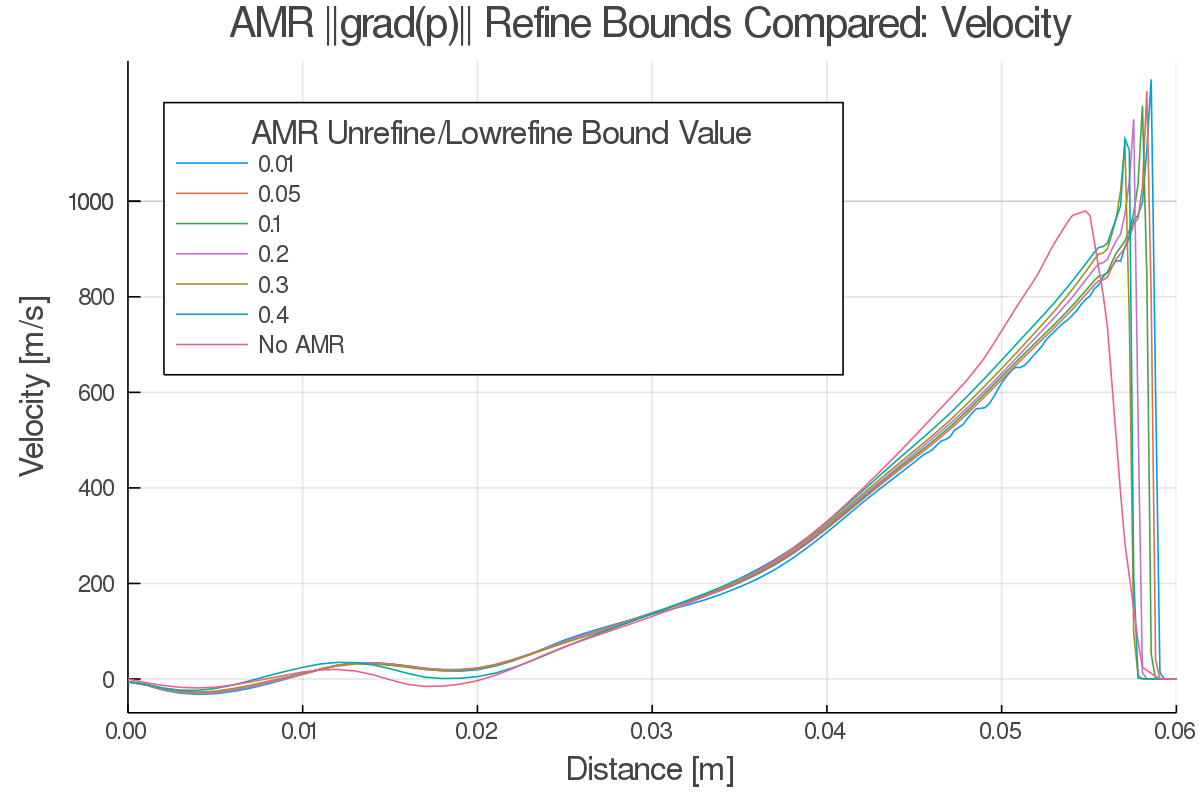
\includegraphics[width=0.9\textwidth]{./figs/amrfigs/amr_refinebounds/u.png}
        \caption{Fluid velocity plot}
    \end{subfigure}

    \centering
    \begin{subfigure}[]{\textwidth}
        \centering
        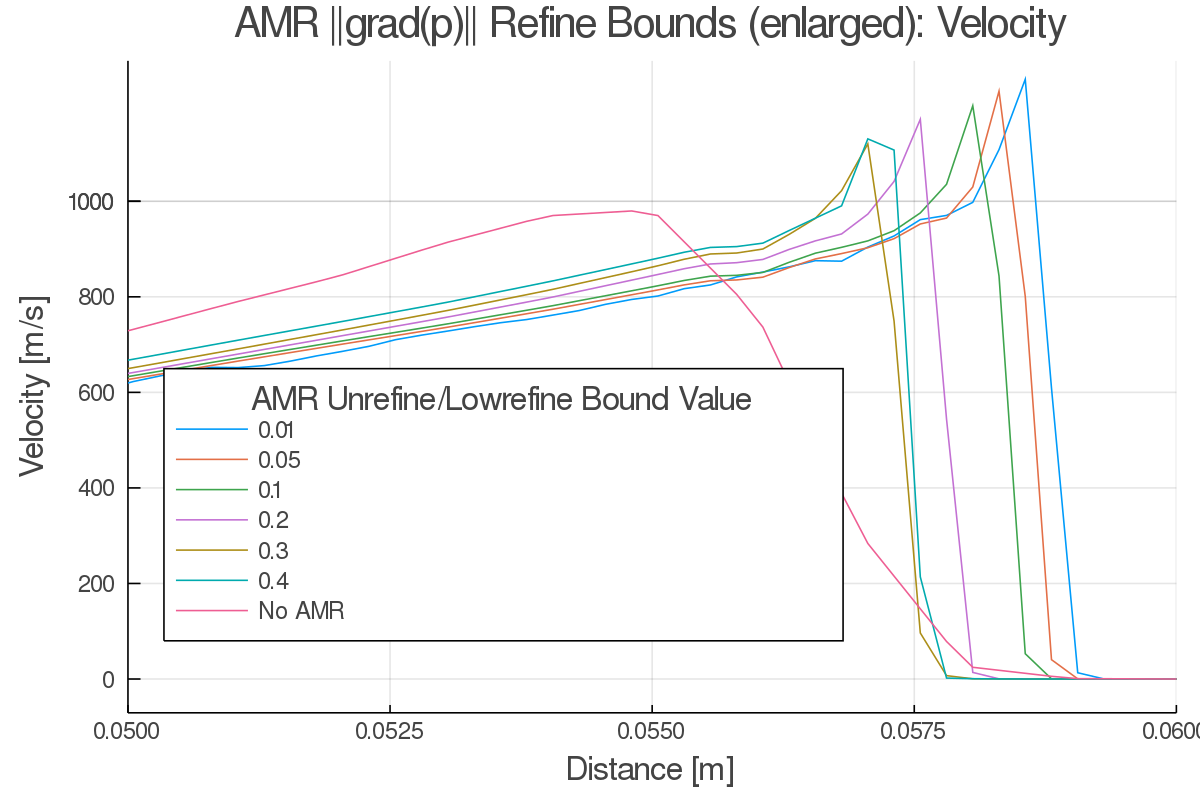
\includegraphics[width=0.9\textwidth]{./figs/amrfigs/amr_refinebounds/ue.png}
        \caption{Fluid velocity plot, enlarged}
    \end{subfigure}

    \caption{Two-dimensional detonation wave AMR results for a 250-40-1 base mesh with 3 refinement levels and 3 buffer layers, tracking \( ||\nabla(p)||\), sweeping refinement bounds }
    \label{fig:amr_refinebounds}
\end{figure}% 
\noindent The static mesh was unchanged from the previous sensitivity plots and the number of refinement levels as well as buffer layers were both 3. It is seen in the figures that by decreasing the refinement bound, the solution increases in accuracy. Pressure values increase the most initially when decreasing the lower bound, up until a lower bound of around 0.1. From here, only further wave propagation is what changes from iteration to iteration. Due to this, 0.1 is the lower bound value that should be selected for PDE and detonation tube modeling if pressure is of interest while keeping the cell count as low as possible for cheaper computation. After this value, the detonation wave location is the parameter that will be affected by further decreases in lower bound of the normalized pressure gradient. If accurate wave location is also of interest (keep in mind that the lowest three refinement bounds, i.e. the most accurate, span around 0.6 mm), then further expansion of the AMR range can be done. Table \ref{tab:amr_refinebounds} contains the cell counts for each lower refinement/unrefinement bound simulation performed in Figure \ref{fig:amr_refinebounds}. It is seen that for this base mesh resolution, a lower bound for the normalized pressure gradient of 0.05 is when the cell count begins to increase considerably. The increase is exponential, so normalized pressure gradient bounds below 0.05 will be more expensive than they are worth. 

\begin{table}[h]
\centering
\caption{Cells for each lower refinement/unrefinement bound for the 250-40-1 simulation at \(t = 3\times 10^{ - 5} s\) in Figure \ref{fig:amr_refinebounds}}
\label{tab:amr_refinebounds}
\begin{tabular}{cc}
Lower refinement/unrefinement bound & Cells \\ \hline
0.01 & 139,136 \\
0.05 & 39,799 \\
0.1 & 38,343 \\ 
0.2 & 37,678 \\
0.3 & 37,692 \\ 
0.4 & 36,355 \\
No AMR & 10,000 \\
\end{tabular}
\end{table}

\section{AMR and Static Comparison}
Various AMR runs were performed, and the best can be found plotted in Figure \ref{fig:amrcompare} along with various comparable static mesh resolutions. Note that due to space, the AMR legend was condensed down and in the following format: [AMR-tracking variable]-[unrefinement level]-[low bound for refinement]-[upper bound for refinement]-[number of buffer layers]-[number of refinement levels]. 
\begin{figure}[]
    \centering
    \begin{subfigure}[]{\textwidth}
        \centering
        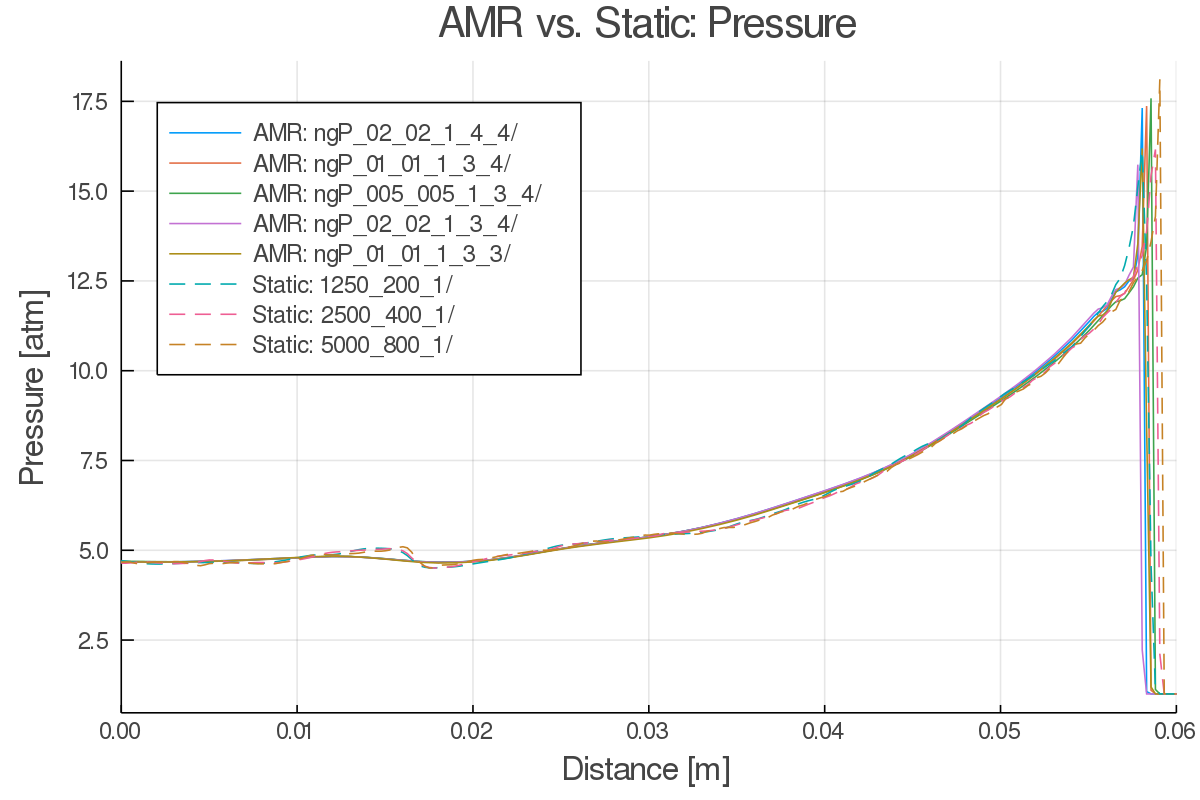
\includegraphics[width=\textwidth]{./figs/amrfigs/amrcompare/p.png}
        \caption{Pressure plot}
    \end{subfigure}

    \centering
    \begin{subfigure}[]{\textwidth}
        \centering
        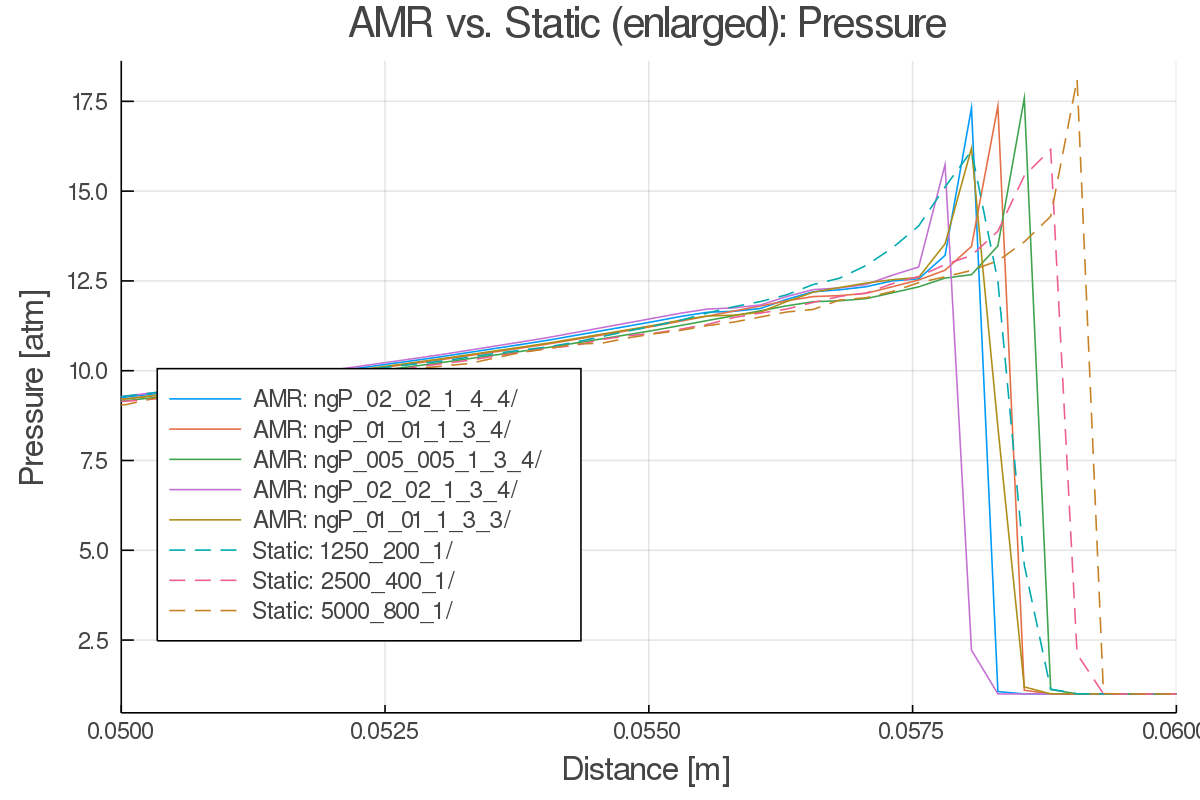
\includegraphics[width=\textwidth]{./figs/amrfigs/amrcompare/pe.png}
        \caption{Pressure plot, enlarged}
    \end{subfigure}

\end{figure}
\begin{figure} \ContinuedFloat

    \centering
    \begin{subfigure}[]{\textwidth}
        \centering
        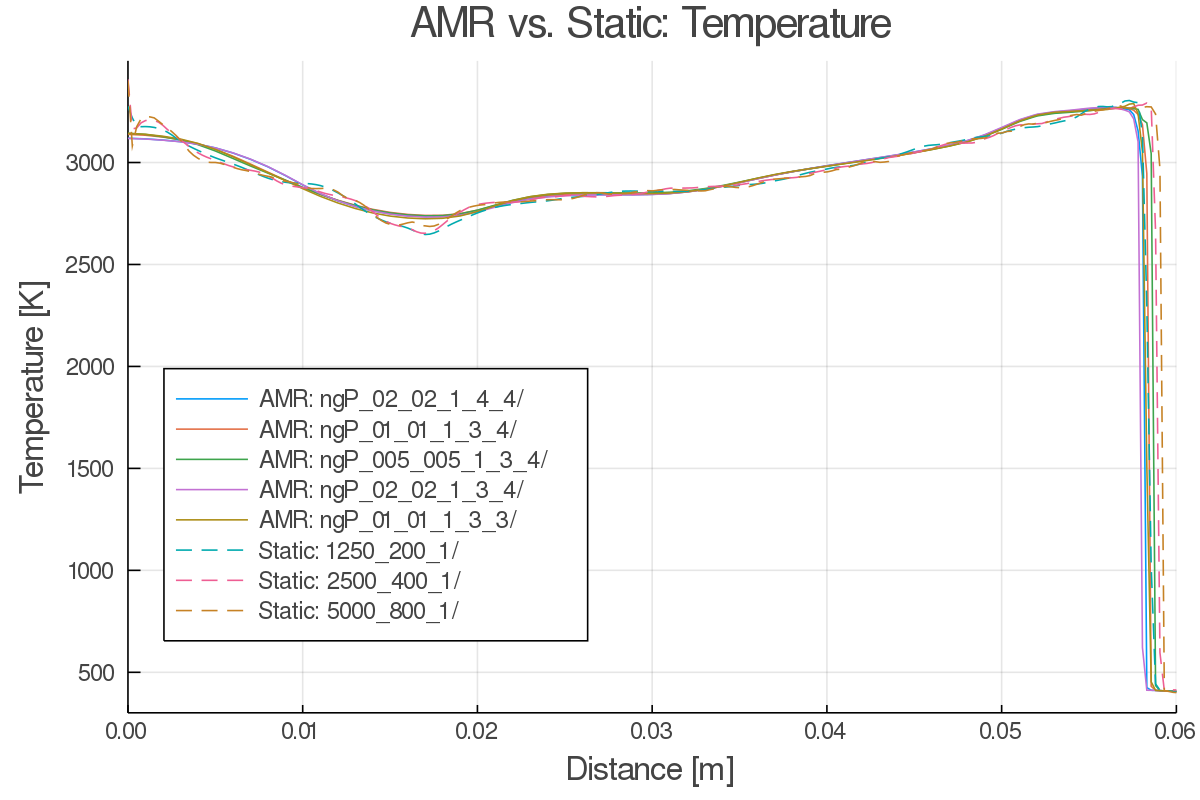
\includegraphics[width=\textwidth]{./figs/amrfigs/amrcompare/t.png}
        \caption{Temperature plot}
    \end{subfigure}

    \centering
    \begin{subfigure}[]{\textwidth}
        \centering
        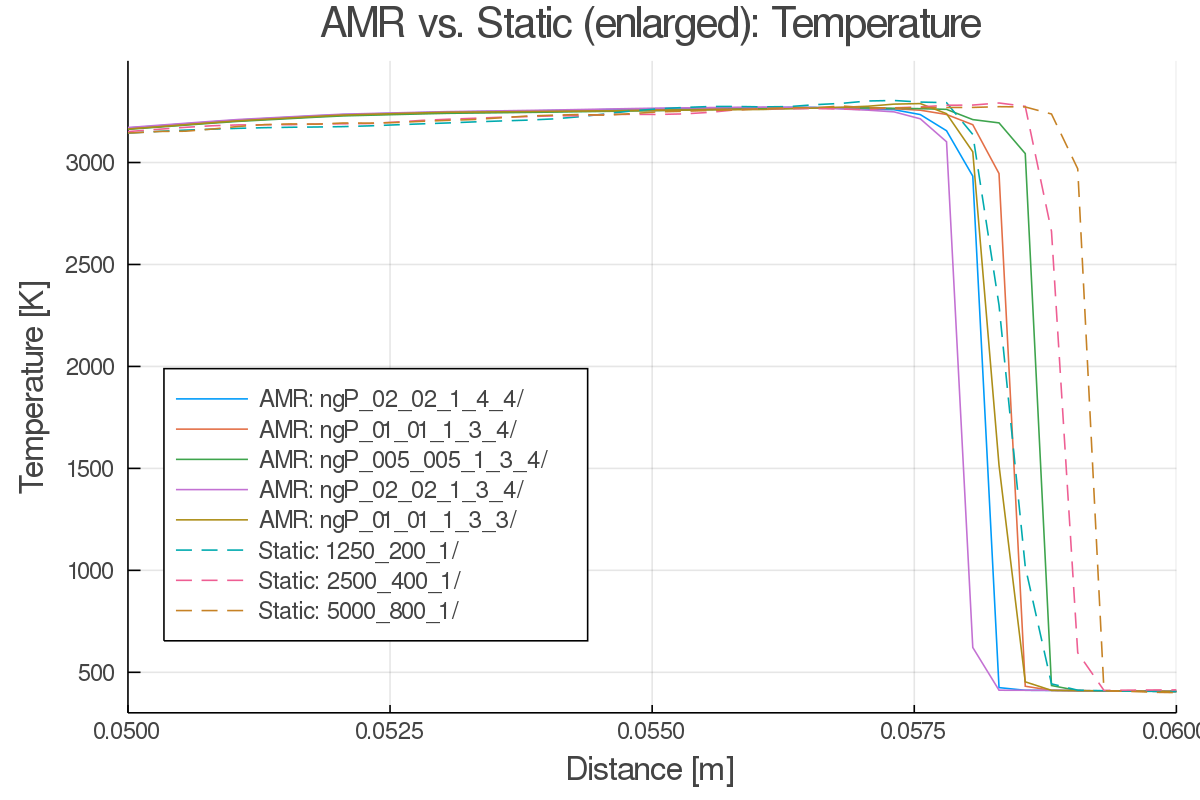
\includegraphics[width=\textwidth]{./figs/amrfigs/amrcompare/te.png}
        \caption{Temperature plot, enlarged}
    \end{subfigure}

\end{figure}
\begin{figure} \ContinuedFloat
    
    \centering
    \begin{subfigure}[]{\textwidth}
        \centering
        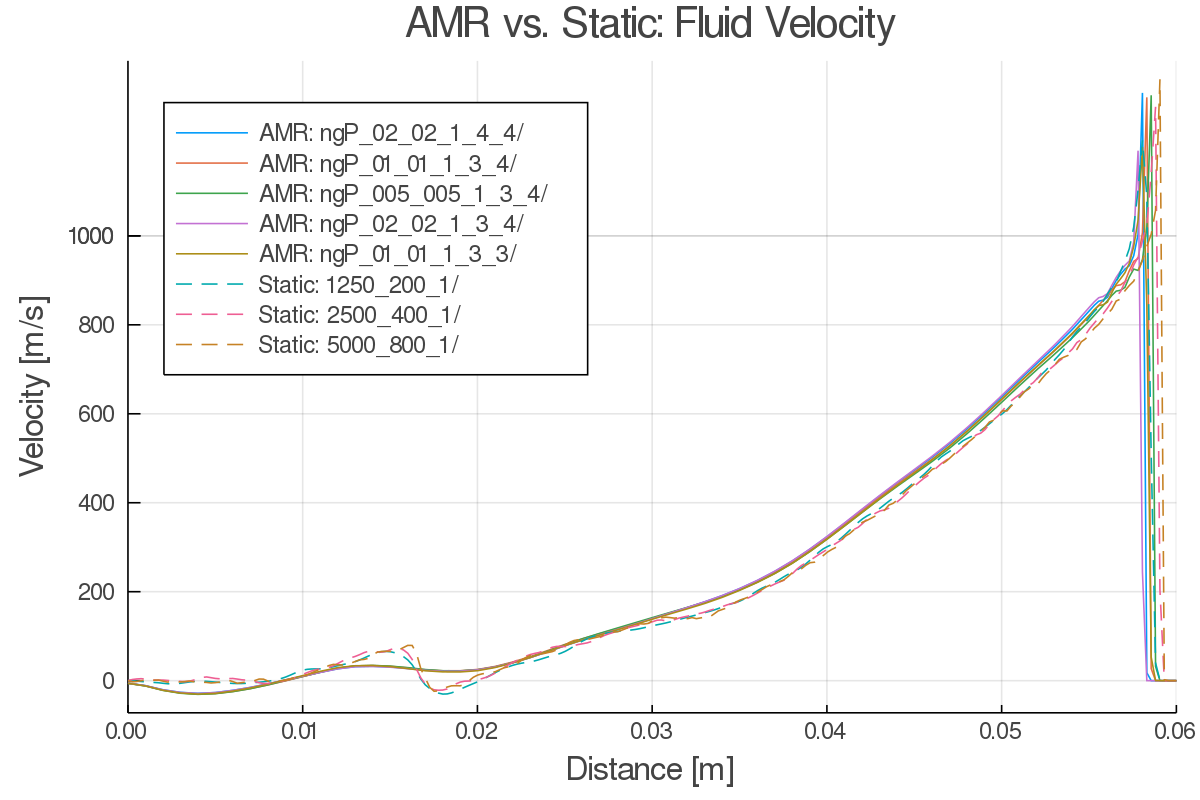
\includegraphics[width=0.9\textwidth]{./figs/amrfigs/amrcompare/u.png}
        \caption{Fluid velocity plot}
    \end{subfigure}

    \centering
    \begin{subfigure}[]{\textwidth}
        \centering
        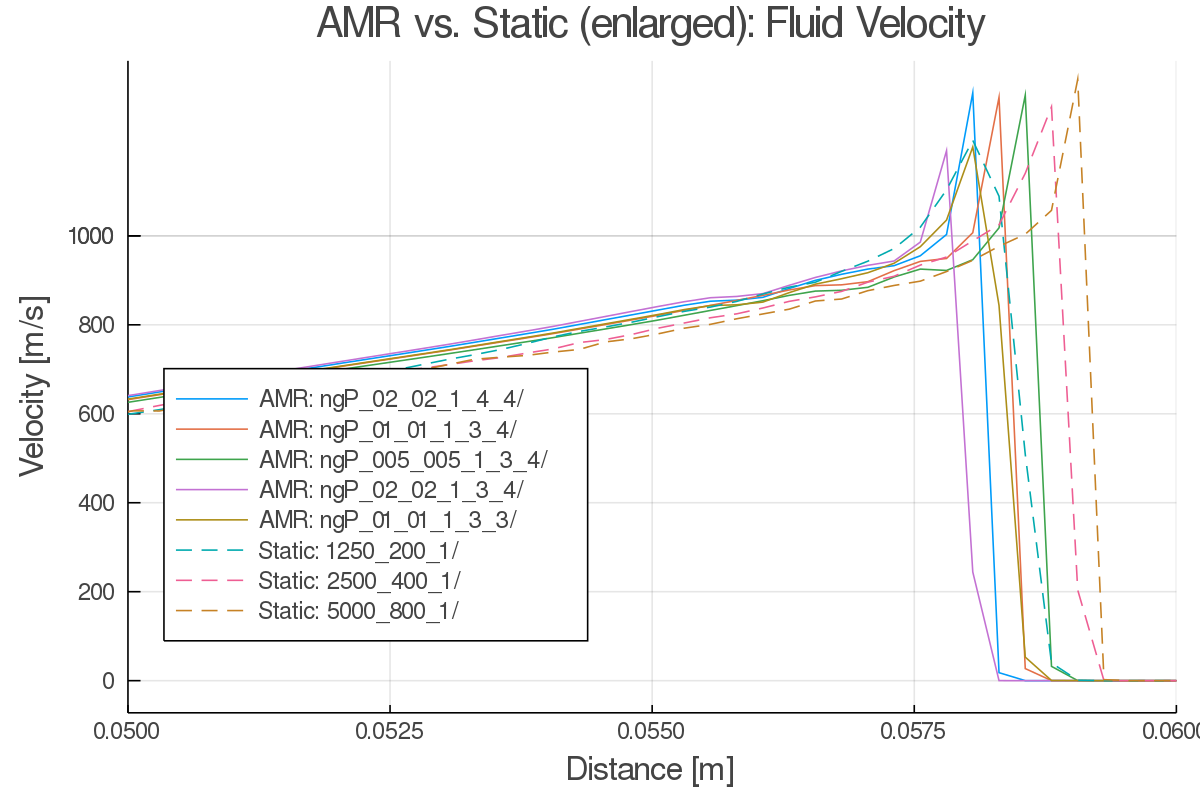
\includegraphics[width=0.9\textwidth]{./figs/amrfigs/amrcompare/ue.png}
        \caption{Fluid velocity plot, enlarged}
    \end{subfigure}

    \caption{Best two-dimensional detonation wave AMR and static mesh results compared, tracking \( ||\nabla(p)||\). AMR legend: field-unrefine-lowrefine-upperrefine-bufferlayers-refinelevels}
    \label{fig:amrcompare}
\end{figure}% 
\noindent Cell counts can be found in Table \ref{tab:amrcompare}. From these plots, a few observations can be made. A very good fit exists between the AMR run with 0.1 for both the unrefine and low refine bound with 3 buffer layers and 3 refinement levels (ngP-01-01-1-3-3) and the static mesh of 1250-200-1. There is an 85\% reduction in cell count between this static mesh and AMR simulation, while exactly reproducing the peak thermodynamic conditions and representing the rest of the detonation profile quite well. 


\begin{table}[h]
\centering
\caption{AMR and Static Mesh Cell Count Comparisons for Figure \ref{fig:amrcompare}, tracking normalized pressure gradient}
\label{tab:amrcompare}
\begin{tabular}{ccp{2cm}p{2cm}p{2cm}p{2cm}c}
Mesh & Type & Unrefine/ lowrefine & Upper ~~~ refine & Buffer ~~ layers & Refine ~~ levels& Cell Count \\ \hline
1250-200-1 & Static & - & - & - & - & 250,000 \\ 
2500-400-1 & Static & - & - & - & - & 1,000,000 \\
5000-800-1 & Static & - & - & - & - & 4,000,000 \\
250-40-1 & AMR & 0.2 & 1 & 4 & 4 & 148,950 \\
250-40-1 & AMR & 0.1 & 1 & 3 & 4 & 149,762 \\
250-40-1 & AMR & 0.05 & 1 & 3 & 4 & 160,570 \\ 
250-40-1 & AMR & 0.2 & 1 & 3 & 4 & 146,710 \\ 
250-40-1 & AMR & 0.1 & 1 & 3 & 3 & 38,343 \\ 
\end{tabular}
\end{table}

If instead we'd like to model the position of the 1250-200-1 static mesh detonation while having more accurate thermodynamic peak temperatures more akin to the 5000-800-1 static mesh, the ngP-02-02-1-4-4 achieves this with 148,950 cells, which is 40\% smaller than the 1250-200-1 static mesh and 96\% smaller than the 5000-800-1 static mesh. A use case where this may be preferable is when you'd like to make sure you're modeling a certain grid resolution entirely, but having a more accurate peak solution would also aid design. Another use scenario of this AMR parameter style is when the position of the detonation wave itself is of less concern but the peak solution values need to still be resolved. 

An important comparison also lies between the ngP-01-01-1-3-3 (solid brown) just mentioned and ngP-02-02-1-3-4 (solid purple) with higher refinement bounds but a single further refinement level AMR runs. While the solid purple simulation has a higher refinement level, the lower normalized pressure gradient bound allows for more cells to be captured around the detonation and model it more accurately while being 3.8 times smaller in terms of number of cells. 
